\title{\textbf{SVD-LLM V2: Explicit Low-Rank Factorization with Trainable Recovery for Transformer Attention Compression}

\author{Anonymous authors}



\section{Introduction}

\subsection{Motivation}

Transformer language models concentrate the majority of their parameters in 
the feed-forward network and multi-head self-attention. In DistilBERT-base, 
the four attention projections $W_Q, W_K, W_V, W_O \in \mathbb{R}^{d \times d}$ 
account for approximately \textbf{70\%} of the parameters in each transformer 
block. Reducing this cost is a high-leverage compression strategy.

\textbf{Low-rank factorization} is the classical primitive. Given a weight matrix 
$W \in \mathbb{R}^{d_\text{out} \times d_\text{in}}$, one replaces it with:

\[
W \approx U \Sigma V^H
\tag{1.1}
\]

where $U \in \mathbb{R}^{d_\text{out} \times r}$, $\Sigma \in \mathbb{R}^{r \times r}$ 
diagonal, and $V^H \in \mathbb{R}^{r \times d_\text{in}}$. The parameter count 
drops from $d_\text{in} d_\text{out}$ to $r(d_\text{in} + d_\text{out} + 1)$.

\textbf{Two design choices.} Prior low-rank methods differ in how they handle the 
singular values:

\begin{enumerate}
\item \textbf{Symmetric factorization.} Store $U \Sigma^{1/2}$ and $\Sigma^{1/2} V^H$
  as two matrices. This balances the factor magnitudes and improves FP16
  stability, but \textbf{loses visibility of $\Sigma$}.
\item \textbf{Explicit factorization.} Store $U$, $\Sigma$, and $V^H$ separately.
  This \textbf{preserves the singular spectrum} for inspection, downstream
  quantization, or spectral analysis.

\end{enumerate}
SVD-LLM V2 adopts the \textbf{explicit} approach. This has three advantages:

\begin{itemize}
\item \textbf{Interpretability.} $\Sigma$ is directly readable and can be visualized.
\item \textbf{Downstream flexibility.} Per-singular-value quantization can be applied
  without re-factorizing.
\item \textbf{Composability.} Orthogonal $U$ and $V^H$ can be re-used across
  checkpoints or merged with other adapters.

\end{itemize}
\subsection{Problem Statement}

Given a pretrained transformer $\mathcal{M}$ with $N_l$ layers and a target 
energy threshold $\eta \in (0, 1)$, we seek a compressed model 
$\mathcal{M}'$ such that:

\[
\mathcal{M}' \approx \mathcal{M}, \qquad
\frac{|\theta(\mathcal{M}')|}{|\theta(\mathcal{M})|} \ll 1
\tag{1.2}
\]

subject to:

\begin{enumerate}
\item \textbf{Explicit factor storage.} Each projection is stored as $U$, $\Sigma$, $V^H$.
\item \textbf{Per-layer adaptive rank.} $r_\ell$ selected by energy threshold.
\item \textbf{Parameter reduction.} $r(d_\text{in} + d_\text{out} + 1) < d_\text{in} d_\text{out}$.
\item \textbf{Multi-architecture support.} Four families (flat, nested, causal, GQA).
\item \textbf{No base retraining.} Only LoRA adapters trained.

\end{enumerate}
\subsection{Our Approach: SVD-LLM V2}

\textbf{SVD-LLM V2} replaces the four attention projections with explicit 
factorized buffers:

\[
W \to (U, \Sigma, V^H), \qquad
y = ((x V^H{}^\top) \Sigma) U^\top + b + \text{LoRA}(x)
\tag{1.3}
\]

The rank is chosen per projection based on spectral energy. LoRA adapters 
$A, B$ are attached with $B = 0$, so the initial output equals the SVD 
approximation.

\textbf{Injection safety.} SVD-LLM V2 combines:
\begin{itemize}
\item \textbf{Pre-test on the first layer} before mutating the model
\item \textbf{Injection-time nested encoder detection}
\item \textbf{Double-injection guard}
\item \textbf{Frobenius norm validation}

\end{itemize}
\textbf{GQA handling.} When the source model has more KV heads than the target 
(e.g., Qwen with $H_{kv} = 2 < H = 8$), K and V weights are **mean-pooled 
per head group** before factorization.

\subsection{Contributions}

\begin{itemize}
\item \textbf{Explicit low-rank factorization.} A variant of SVD compression that
  keeps $U$, $\Sigma$, $V^H$ separate, preserving interpretability and
  enabling downstream flexibility.
\item \textbf{Energy-threshold rank selection.} Per-projection rank chosen by
  cumulative spectral energy.
\item \textbf{Multi-architecture hardening.} Four families with pre-test, injection-time
  nested detection, and GQA pooling.
\item \textbf{A systematic evaluation.} Benchmark on three models on SST-2 with
  ablations over $r_\text{max}$, $\eta$, and LoRA rank.
\item \textbf{Full reproducibility.} Code, checkpoints, and scripts released under
  Apache 2.0.

\end{itemize}
\subsection{Relationship to Prior Work}

SVD-LLM V2 is a continuation of the \textbf{SVD-LLM} line:

\begin{table}[H]
\centering
\small
\begin{tabular}{ll}
\toprule
\textbf{Version} & \textbf{Main features} \\
\midrule
SVD-LLM V1 & Basic SVD compression \\
\textbf{SVD-LLM V2} & Explicit U/$\Sigma$/V\^{}H + LoRA + multi-arch hardening \\
\bottomrule
\end{tabular}
\end{table}

It also compares to the \textbf{Minimal family} (MinimalSVD, MinimalNOVA, 
MinimalPRISM) which use symmetric factorization:

\begin{table}[H]
\centering
\small
\begin{tabular}{lll}
\toprule
\textbf{Family} & \textbf{Factorization} & \textbf{Interpretable?} \\
\midrule
Minimal family & $U\sqrt{\Sigma} \cdot \sqrt{\Sigma} V^H$ & No \\
\textbf{SVD-LLM V2} & $U \cdot \Sigma \cdot V^H$ (separate) & \textbf{Yes} \\
\bottomrule
\end{tabular}
\end{table}

\subsection{Paper Organization}

Section 2 reviews related work. Section 3 provides background. Section 4 
presents SVD-LLM V2. Section 5 describes architecture integration. Section 6 
details the setup. Section 7 reports results. Section 8 analyzes the 
explicit-factor approach. Section 9 discusses guidance. Section 10 lists 
limitations. Section 11 concludes.



\subsection{Notation}

\begin{lstlisting}

---
\end{lstlisting}


\section{Related Work}

\subsection{Low-Rank Matrix Factorization}

\textbf{Classical SVD.} The Eckart--Young theorem (Eckart \& Young, 1936) states 
that the best rank-$r$ approximation of $W$ in Frobenius norm is the 
truncated SVD. SVD-LLM V2 uses this as the core primitive.

\textbf{Symmetric vs. explicit factorization.} Standard implementations distribute 
$\Sigma^{1/2}$ between $U$ and $V^H$ (Golub \& Van Loan, 2013). SVD-LLM V2 
instead keeps $\Sigma$ separate, sacrificing FP16 stability for 
interpretability.

\textbf{Randomized SVD.} Halko et al. (2011) provide randomized algorithms. For 
our layer sizes, exact SVD is feasible.

\textbf{Weighted low-rank.} Golub et al. (1987) and Srebro \& Jaakkola (2003) study 
weighted variants. Activation-aware methods (Lin et al., 2023; Xiao et al., 
2023) use activation statistics. SVD-LLM V2 uses unweighted SVD with 
energy-adaptive rank.

\subsection{Rank Selection Strategies}

\textbf{Fixed rank.} Most methods use a global $r$ (Yu et al., 2017).

\textbf{AdaLoRA.} Zhang et al. (2023) learn per-layer rank budgets. SVD-LLM V2 
uses a fixed \textbf{energy threshold}, simpler and training-free.

\textbf{Energy-based truncation.} Standard in signal processing. SVD-LLM V2 
applies it to transformer attention.

\subsection{Parameter-Efficient Fine-Tuning}

\textbf{LoRA.} Hu et al. (2021) freeze base weights and train rank-$r$ adapters. 
SVD-LLM V2 uses LoRA as the recovery mechanism.

\textbf{DoRA.} Liu et al. (2024) decompose weights into magnitude and direction. 
Related in spirit to explicit $\Sigma$ storage.

\subsection{Attention Variants}

\textbf{Standard MHSA.} Vaswani et al. (2017) introduce the four-projection 
attention. SVD-LLM V2 preserves the four-projection structure.

\textbf{GQA.} Ainslie et al. (2023) share KV heads. SVD-LLM V2 supports GQA via 
mean-pooling of K and V weights.

\textbf{MQA.} Shazeer (2019) uses a single KV head. Compatible.

\subsection{Model Compression}

\begin{table}[H]
\centering
\small
\begin{tabular}{lllll}
\toprule
\textbf{Method} & \textbf{Type} & \textbf{Ratio} & \textbf{Retrain} & \textbf{Interpretable?} \\
\midrule
DistilBERT & Distillation & 1.6$$\times$ & Yes & No \\
SparseGPT & Pruning & 2-4$$\times$ & No & Partial \\
AWQ & Quantization & 4$$\times$ & No & No \\
A3 & Low-rank + Fisher & 5$$\times$ & LoRA & No \\
AASVD & Low-rank + covariance & 5$$\times$ & LoRA & No \\
MinimalSVD & Low-rank + energy & 3-6$$\times$ & LoRA & No \\
\textbf{SVD-LLM V2} & \textbf{Low-rank + explicit $\Sigma$} & \textbf{50\%$$\times$} & \textbf{LoRA} & \textbf{Yes} \\
\bottomrule
\end{tabular}
\end{table}

\subsection{Position of Our Work}

SVD-LLM V2 differs from prior work along three axes:

\begin{table}[H]
\centering
\small
\begin{tabular}{lll}
\toprule
\textbf{Axis} & \textbf{Prior} & \textbf{SVD-LLM V2} \\
\midrule
\textbf{Factorization} & Symmetric & \textbf{Explicit (U, $\Sigma$, V\^{}H)} \\
\textbf{Interpretability} & Limited & \textbf{Full} \\
\textbf{Downstream flexibility} & Low & \textbf{High} \\
\bottomrule
\end{tabular}
\end{table}

\textbf{Key distinction.} Unlike symmetric-factorization methods, SVD-LLM V2 
preserves the singular spectrum for inspection and downstream applications 
(e.g., per-singular-value quantization, spectral analysis). This comes at 
the cost of slight numerical sensitivity in FP16.



\subsection{Comparison with Companion Methods}

\begin{lstlisting}

---
\end{lstlisting}


\section{Background}

\subsection{Singular Value Decomposition}

For $W \in \mathbb{R}^{m \times n}$:

\[
W = U \Sigma V^H
\tag{3.1}
\]

where $U \in \mathbb{R}^{m \times m}$, $V \in \mathbb{R}^{n \times n}$ are 
unitary, and $\Sigma \in \mathbb{R}^{m \times n}$ is diagonal with 
$\sigma_1 \geq \sigma_2 \geq \dots \geq 0$.

\textbf{Truncated SVD.} Keeping the top-$r$:

\[
W_r = U_{:, :r} \Sigma_{:r, :r} V_{:r, :}^H
\tag{3.2}
\]

\textbf{Optimality.} By Eckart--Young, $W_r$ minimizes $\|W - W_r\|_F$. Error:

\[
\|W - W_r\|_F = \sqrt{\sum_{i > r} \sigma_i^2}
\tag{3.3}
\]

\textbf{Symmetric form (common).} Many implementations store $U\Sigma^{1/2}$ and 
$\Sigma^{1/2}V^H$ for FP16 stability:

\[
W_r = \underbrace{U_{:, :r}\Sigma_{:r, :r}^{1/2}}_{\text{factor 1}} \cdot \underbrace{\Sigma_{:r, :r}^{1/2}V_{:r, :}^H}_{\text{factor 2}}
\tag{3.4}
\]

\textbf{Explicit form (SVD-LLM V2).} SVD-LLM V2 stores $U$, $\Sigma$, $V^H$ 
\textbf{separately}:

\[
W_r = U_{:, :r} \cdot \Sigma_{:r, :r} \cdot V_{:r, :}^H
\tag{3.5}
\]

This is less numerically stable but \textbf{interpretable}.

\subsection{Cumulative Spectral Energy}

\[
E(r) = \frac{\sum_{i \leq r} \sigma_i^2}{\sum_i \sigma_i^2}
\tag{3.6}
\]

$E(r)$ is monotonically increasing from $0$ to $1$.

\textbf{Energy threshold.} Given $\eta$:

\[
r_\text{eff} = \min\{r : E(r) \geq \eta\}
\tag{3.7}
\]

\subsection{Multi-Head Self-Attention}

For input $X \in \mathbb{R}^{B \times L \times d}$:

\[
\begin{aligned}
Q &= X W_Q, \quad K = X W_K, \quad V = X W_V \\
\text{head}_h &= \text{softmax}\!\left(\frac{Q_h K_h^\top}{\sqrt{d_h}}\right) V_h \\
\text{MHSA}(X) &= \text{Concat}(\text{head}_1, \dots, \text{head}_H) W_O
\end{aligned}
\tag{3.8}
\]

\subsection{Grouped-Query Attention (GQA)}

$H_{kv} < H$ KV heads. Repeated $H / H_{kv}$ times. SVD-LLM V2 factorizes at 
natural dimensions and applies \texttt{repeat\_kv} at forward.

\subsection{GQA Weight Pooling}

When the source model has more KV heads than the target dimension, we 
\textbf{mean-pool} per group:

\[
W_K^\text{pooled}_{h, :} = \frac{1}{|G_h|} \sum_{g \in G_h} W_{g, :}
\tag{3.9}
\]

where $G_h$ is the group of source heads mapped to target head $h$. This is 
used when loading a checkpoint trained with a different head count.

\subsection{Rotary Position Embeddings (RoPE)}

RoPE (Su et al., 2021) rotates $Q, K$:

\[
\tilde{Q}_i = Q_i \cos(\theta_i) + \text{rot}(Q_i) \sin(\theta_i)
\tag{3.10}
\]

SVD-LLM V2 applies RoPE after projection, preserving structure.

\subsection{LoRA Recovery}

LoRA (Hu et al., 2021):

\[
\Delta W = \frac{\alpha}{r_L} B A
\tag{3.11}
\]

with $B = 0$ at initialization. In SVD-LLM V2:

\[
y = ((x V^H{}^\top) \Sigma) U^\top + (x A^\top) B^\top \cdot s + b
\tag{3.12}
\]

\subsection{Nested Encoder Structure}

In BERT-style models:

\begin{lstlisting}
BertAttention
+-- self       (BertSelfAttention)
|   +-- query
|   +-- key
|   +-- value
+-- output     (BertSelfOutput)
    +-- dense  # $\leftarrow$ Output projection OUTSIDE
\end{lstlisting}

SVD-LLM V2 sets \texttt{is\_nested\_encoder = True} and skips \texttt{out\_proj} in forward.

\subsection{Conv1D in GPT-2}

GPT-2 uses HuggingFace \texttt{Conv1D}, storing \texttt{(in, out)}:

\begin{lstlisting}
self.weight = nn.Parameter(torch.empty(nx, nf))  # (in, out)
\end{lstlisting}

SVD-LLM V2 transposes via \texttt{\_unpack\_weight\_bias}.

\subsection{Notation Summary}

\begin{lstlisting}

---
\end{lstlisting}


\section{Method}

\subsection{Overview}

SVD-LLM V2 replaces each attention projection with **three explicit 
buffers**:

\[
W \to (U, \Sigma, V^H)
\tag{4.1}
\]

The forward pass computes:

\[
y = ((x V^H{}^\top) \Sigma) U^\top + b + \text{LoRA}(x)
\tag{4.2}
\]

Rank is chosen per projection by energy threshold. LoRA adapters provide 
recovery.

\textbf{Figure 4.1} shows the pipeline.

\begin{lstlisting}
   +----------------------------------------------+
   |  Input weight W $\in$ R^{d_out $$\times$ d_in}           |
   +--------------------+-------------------------+
                        |
                         
   +----------------------------------------------+
   |  SVD: W = U $\Sigma$ V^H                             |
   |  Compute cumulative energy E(r)              |
   |  r_eff = min(r_max, argmin E(r) $\ge$  )         |
   +--------------------+-------------------------+
                        |
                         
   +----------------------------------------------+
   |  Store explicitly:                            |
   |  U  $\in$ R^{d_out $$\times$ r}                           |
   |  $\Sigma$  $\in$ R^r (diagonal)                          |
   |  V^H $\in$ R^{r $$\times$ d_in}                           |
   +--------------------+-------------------------+
                        |
                         
   +----------------------------------------------+
   |  Freeze U, $\Sigma$, V^H. Add LoRA (A, B=0)          |
   +----------------------------------------------+
\end{lstlisting}

\subsection{The Explicit Factor Buffers}

For each projection (Q, K, V, out), we allocate:

\begin{table}[H]
\centering
\small
\begin{tabular}{lll}
\toprule
\textbf{Buffer} & \textbf{Shape} & \textbf{Purpose} \\
\midrule
\texttt{*\_u} & $(d_\text{out}, r)$ & Left singular vectors \\
\texttt{*\_s} & $(r,)$ & Singular values (1D) \\
\texttt{*\_vh} & $(r, d_\text{in})$ & Right singular vectors \\
\texttt{*\_bias} & $(d_\text{out},)$ & Bias (separate) \\
\bottomrule
\end{tabular}
\end{table}

Where \texttt{*} is one of \texttt{query}, \texttt{key}, \texttt{value}, \texttt{out\_proj}.

\textbf{Memory savings.} For $d = 768$ and $r = 128$:

\begin{table}[H]
\centering
\small
\begin{tabular}{ll}
\toprule
\textbf{Config} & \textbf{Params} \\
\midrule
Original & 589,824 \\
Explicit (U + $\Sigma$ + V\^{}H) & $768 \times 128 + 128 + 128 \times 768 = 196{,}736$ \\
Ratio & \textbf{3.0$$\times$} \\
\bottomrule
\end{tabular}
\end{table}

With rank 64: \textbf{6.0$$\times$} reduction.

\subsection{The `\_project` Helper}

SVD-LLM V2 uses a unified helper:

\begin{lstlisting}
def _project(self, x, vh, s, u, b, lora_A, lora_B):
    base_out = ((x @ vh.t()) * s.to(dtype=x.dtype)) @ u.t() + b
    if self.lora_rank > 0 and lora_A is not None and lora_B is not None:
        lora_out = F.linear(F.linear(x, lora_A), lora_B) * self.scaling
        base_out = base_out + lora_out
    return base_out
\end{lstlisting}

\textbf{Order of operations:}

\begin{enumerate}
\item Down-project: $x V^H{}^\top$ $\to$ $(B, L, r)$
\item Scale: multiply by $\Sigma$ $\to$ $(B, L, r)$
\item Up-project: $\cdot U^\top$ $\to$ $(B, L, d_\text{out})$
\item Add bias
\item Add LoRA residual

\end{enumerate}
\subsection{Energy-Threshold Rank Selection}

Given $W$, target rank cap $r_\text{max}$, and energy $\eta$:

\begin{enumerate}
\item Compute SVD: $W = U \Sigma V^H$.
\item Compute cumulative energy: $E(r) = \sum_{i \leq r} \sigma_i^2 / \sum_i \sigma_i^2$.
\item Find: $r_\text{energy} = |\{i : E(i) < \eta\}| + 1$.
\item Cap: $r_\text{eff} = \min(r_\text{energy}, r_\text{max}, \min(d_\text{in}, d_\text{out}))$.

\end{enumerate}
The rank is set \textbf{per projection} (not per layer). This means Q, K, V, out 
may each get a different rank.

\subsection{Weight Transfer}

\subsubsection{Architecture Patterns}

\begin{table}[H]
\centering
\small
\begin{tabular}{ll}
\toprule
\textbf{Architecture} & \textbf{Extraction} \\
\midrule
GPT-2 & Split \texttt{c\_attn} into 3 chunks; separate \texttt{c\_proj} \\
RoBERTa & Extract \texttt{self.query/key/value} and \texttt{output.dense} \\
Qwen & Extract \texttt{q\_proj/k\_proj/v\_proj} and \texttt{o\_proj} \\
DistilBERT & Extract \texttt{q\_lin/k\_lin/v\_lin} and \texttt{out\_lin} \\
Fallback & UniversalAdapter \\
\bottomrule
\end{tabular}
\end{table}

\subsubsection{Conv1D Handling}

\begin{lstlisting}
def _unpack_weight_bias(module):
    base = getattr(module, "base_layer", module)
    w = base.weight.data.clone()
    if "Conv1D" in type(module).__name__ or hasattr(module, "nf"):
        w = w.t()   # (in, out) $\to$ (out, in)
    return w, base.bias
\end{lstlisting}

\subsubsection{GQA Pooling}

When \texttt{w\_k.shape[0] != self.kv\_head\_size}:

\begin{lstlisting}
rep = w_k.shape[0] // self.kv_head_size
w_k_pooled = (
    w_k.view(self.num_kv_heads, rep, self.head_dim, -1)
    .mean(dim=1)
    .view(self.kv_head_size, -1)
)
\end{lstlisting}

Same for bias.

\subsection{Nested Encoder Detection}

\texttt{is\_nested\_encoder} is set based on the presence of \texttt{src.self.query}:

\begin{lstlisting}
if hasattr(src, "self") and hasattr(getattr(src, "self"), "query"):
    # Nested encoder -- extract from inner, skip out_proj
    w_o = src.output.dense.weight
    self.is_nested_encoder = True
\end{lstlisting}

When nested, \texttt{out\_proj} is skipped in forward.

\subsection{Injection Protocol}

\textbf{Algorithm 1:} Whole-model injection with pre-test
\begin{lstlisting}
Input:  model M, rank cap r_max, energy  
Output: M' with factorized attention

1:  layer_list $\leftarrow$ find_transformer_layers(M)
2:
3:  # Pre-test on first layer
4:  test_src $\leftarrow$ get_attention(layer_list[0])
5:  try:
6:      test_module $\leftarrow$ SVDLLMV2Attention(cfg, old_attn=test_src)
7:  except Exception:
8:      return None
9:
10: # Inject each layer
11: count $\leftarrow$ 0
12: for (idx, layer) in enumerate(layer_list) do
13:     src_attn $\leftarrow$ get_attention(layer)
14:     if src_attn is SVDLLMV2Attention: skip
15:     new_attn $\leftarrow$ SVDLLMV2Attention(cfg, old_attn=src_attn)
16:
17:     # Set nested flag and replace
18:     for attr in ("attention", "attn", "self_attn", "self"):
19:         if hasattr(layer, attr):
20:             if attr == "attention" and hasattr(layer.attention, "self"):
21:                 new_attn.is_nested_encoder = True
22:                 layer.attention.self = new_attn
23:             else:
24:                 new_attn.is_nested_encoder = False
25:                 setattr(layer, attr, new_attn)
26:             break
27:     count += 1
28: end for
29:
30: return M' if count > 0 else None
\end{lstlisting}

\subsection{LoRA Recovery}

Each projection has its own LoRA pair:

\begin{itemize}
\item \texttt{q\_lora\_A}, \texttt{q\_lora\_B}
\item \texttt{k\_lora\_A}, \texttt{k\_lora\_B}
\item \texttt{v\_lora\_A}, \texttt{v\_lora\_B}
\item \texttt{out\_lora\_A}, \texttt{out\_lora\_B}

\end{itemize}
All \texttt{*\_B} are initialized to zero. Base weights ($U$, $\Sigma$, $V^H$, biases) 
are frozen.

\subsection{Complexity Analysis}

\begin{table}[H]
\centering
\small
\begin{tabular}{lll}
\toprule
\textbf{Phase} & \textbf{Time} & \textbf{Memory} \\
\midrule
Extraction & $\mathcal{O}(N_l d^2)$ & $\mathcal{O}(d^2)$ \\
SVD per projection & $\mathcal{O}(d^3)$ & $\mathcal{O}(d^2)$ \\
Truncation & $\mathcal{O}(N_l r d^2)$ & $\mathcal{O}(d^2)$ \\
Total & $\mathcal{O}(N_l d^3)$ & $\mathcal{O}(d^2)$ \\
\bottomrule
\end{tabular}
\end{table}

\subsection{Theoretical Notes}

\subsubsection{Energy Bound}

\textbf{Proposition.} If $r_\text{eff}$ is the smallest rank with 
$E(r_\text{eff}) \geq \eta$, then:

\[
\frac{\|W - W_{r_\text{eff}}\|_F}{\|W\|_F} \leq \sqrt{1 - \eta}
\tag{4.3}
\]

\textbf{Proof.} $\|W - W_r\|_F^2 = \|W\|_F^2 (1 - E(r))$. $\square$

\subsubsection{Explicit vs Symmetric Factorization}

Both forms are mathematically equivalent:

\[
(U \Sigma^{1/2}) (\Sigma^{1/2} V^H) = U \Sigma V^H
\tag{4.4}
\]

The explicit form exposes $\Sigma$ for interpretation. The symmetric form is 
numerically stabler in FP16 because both factors have unit spectral norm.

\textbf{SVD-LLM V2 default:} explicit. For FP16-only deployments, consider 
switching to symmetric.

\subsection{Summary}

SVD-LLM V2:
\begin{enumerate}
\item Factorizes each attention projection into explicit $(U, \Sigma, V^H)$.
\item Selects rank per projection via energy threshold.
\item Uses LoRA for recovery.
\item Handles four attention architectures with pre-test and GQA pooling.
\item Achieves \textbf{real parameter reduction} of $d^2 / (r(d_\text{in} + d_\text{out} + 1))$.
\end{enumerate}
\begin{lstlisting}

---
\end{lstlisting}


\section{Architecture Integration}

\subsection{Model Support}

\begin{table}[H]
\centering
\small
\begin{tabular}{lllllll}
\toprule
\textbf{Model} & \textbf{Layers} & \textbf{$d$} & \textbf{$H$} & \textbf{$H_{kv}$} & \textbf{Nested?} & \textbf{Conv1D?} \\
\midrule
DistilBERT-base & 6 & 768 & 12 & 12 & No & No \\
RoBERTa-base & 12 & 768 & 12 & 12 & Yes & No \\
GPT-2 & 12 & 768 & 12 & 12 & No & Yes \\
Qwen3.5-0.8B & 24 & 1024 & 8 & 2 & No & No \\
\bottomrule
\end{tabular}
\end{table}

\subsection{DistilBERT (Flat)}

\begin{lstlisting}
distilbert.transformer.layer.0.attention
+-- q_lin  (Linear 768 $\to$ 768)
+-- k_lin  (Linear 768 $\to$ 768)
+-- v_lin  (Linear 768 $\to$ 768)
+-- out_lin (Linear 768 $\to$ 768)
\end{lstlisting}

All four are \texttt{nn.Linear}. Direct factorization.

\texttt{is\_nested\_encoder = False} because \texttt{out\_lin} is inside the attention.

\subsection{RoBERTa (Nested)}

\begin{lstlisting}
roberta.encoder.layer.0.attention
+-- self
|   +-- query
|   +-- key
|   +-- value
+-- output
    +-- dense  # $\leftarrow$ outside
\end{lstlisting}

\textbf{Critical:} \texttt{output.dense} sits outside. SVD-LLM V2 sets 
\texttt{is\_nested\_encoder = True} and skips \texttt{out\_proj}.

\textbf{Detection.} In \texttt{copy\_weights}:

\begin{lstlisting}
if hasattr(old_attn, "self") and hasattr(old_attn, "output"):
    src = old_attn.self
    if hasattr(old_attn.output, "dense"):
        w_o, b_o = _unpack_weight_bias(old_attn.output.dense)
    # Note: even though we extract W_O, we set is_nested_encoder=True
    # so it will NOT be used in forward.
\end{lstlisting}

Wait -- SVD-LLM V2 \textbf{does} extract \texttt{W\_O} from the outer layer but **skips 
it** in forward if nested. This may seem redundant but keeps the code 
uniform. In our experiments, this extraction is only used to validate 
weight availability; the actual out projection is applied by the outer 
\texttt{BertSelfOutput.dense}.

\subsection{GPT-2 (Causal Conv1D)}

\begin{lstlisting}
transformer.h.0.attn
+-- c_attn  (Conv1D 768 $\to$ 2304)   # fused Q, K, V
+-- c_proj  (Conv1D 768 $\to$ 768)
\end{lstlisting}

\textbf{Split c\_attn:}

\begin{lstlisting}
c_attn_w, c_attn_b = _unpack_weight_bias(src.c_attn)
split_size = c_attn_w.size(0) // 3
w_q = c_attn_w[:split_size, :]
w_k = c_attn_w[split_size : 2 * split_size, :]
w_v = c_attn_w[2 * split_size :, :]
\end{lstlisting}

\textbf{Conv1D transposition:} \texttt{\_unpack\_weight\_bias} handles this automatically:

\begin{lstlisting}
if "Conv1D" in type(module).__name__ or hasattr(module, "nf"):
    w = w.t()
\end{lstlisting}

\texttt{is\_nested\_encoder = False} because \texttt{c\_proj} is inside the attention.

\subsection{Qwen3.5 (GQA + RoPE)}

\begin{lstlisting}
model.layers.0.self_attn
+-- q_proj  (Linear 1024 $\to$ 2048)   # H * d_h
+-- k_proj  (Linear 1024 $\to$ 512)    # H_kv * d_h
+-- v_proj  (Linear 1024 $\to$ 512)
+-- o_proj  (Linear 2048 $\to$ 1024)
\end{lstlisting}

\textbf{GQA pooling.} When source \texttt{W\_K} has more rows than \texttt{self.kv\_head\_size}:

\begin{lstlisting}
rep = w_k.shape[0] // self.kv_head_size
w_k_pooled = (
    w_k.view(self.num_kv_heads, rep, self.head_dim, -1)
    .mean(dim=1)
    .view(self.kv_head_size, -1)
)
\end{lstlisting}

\textbf{RoPE handling.} Qwen passes \texttt{position\_embeddings} in kwargs. SVD-LLM V2 
applies RoPE after projection.

\texttt{is\_nested\_encoder = False}.

\subsection{Nested Encoder Bypass}

When \texttt{is\_nested\_encoder = True}:

\begin{lstlisting}
context = torch.matmul(probs, V).transpose(1, 2).contiguous().view(...)

if self.is_nested_encoder:
    out = context       # $\leftarrow$ No out_proj
else:
    out = self._project(context, ...)   # $\leftarrow$ out_proj applied
\end{lstlisting}

The outer \texttt{BertSelfOutput.dense} then applies the projection.

\subsection{Injection Protocol}

SVD-LLM V2's injection hook has three safety layers:

\subsubsection{Pre-Test}

\begin{lstlisting}
test_src = layer_list[0].attention
try:
    test_module = SVDLLMV2Attention(cfg, old_attn=test_src, ...)
except Exception as e:
    logger.warning(f"Pre-test failed: {e}")
    return None
\end{lstlisting}

\subsubsection{Double-Injection Guard}

\begin{lstlisting}
if isinstance(src, SVDLLMV2Attention) or "SVDLLMV2" in src.__class__.__name__:
    return None
\end{lstlisting}

\subsubsection{Frobenius Validation}

\begin{lstlisting}
for name, w in [("w_q", w_q), ("w_k", w_k), ("w_v", w_v)]:
    if torch.norm(w.float(), p="fro").item() < 1e-4:
        raise RuntimeError(f"Near-zero norm on {name}")
\end{lstlisting}

\subsection{Failure Modes and Fallbacks}

\begin{table}[H]
\centering
\small
\begin{tabular}{lll}
\toprule
\textbf{Failure} & \textbf{Detection} & \textbf{Response} \\
\midrule
Missing weights & Pre-test or \texttt{copy\_weights} raises & Abort injection \\
Near-zero Frobenius & Norm check < 1e-4 & Raise \\
Shape mismatch & Padding in \texttt{\_decompose\_and\_set} & Warn \\
Double injection & Class name guard & Skip \\
Cross-attention & Not supported & Not implemented \\
\bottomrule
\end{tabular}
\end{table}

\subsection{Registry}

\begin{lstlisting}
@ATTENTION_REGISTRY.register("svd_llm_v2")
@ATTENTION_REGISTRY.register("svd_llm_v2_attention")
class SVDLLMV2Attention(BaseAttention):
    ...

@ATTENTION_REGISTRY.register("svd_llm_v2_inject")
@ATTENTION_REGISTRY.register("inject_svd_llm_v2")
def inject_svd_llm_v2(...):
    ...
\end{lstlisting}

\subsection{Interaction with LoRA Recovery Pipeline}

SVD-LLM V2 integrates cleanly with the framework's LoRA recovery:

\begin{enumerate}
\item \textbf{Inject} SVD-LLM V2 $\to$ explicit factor buffers, frozen.
\item \textbf{LoRA adapters} per projection (q/k/v/out) are trainable.
\item \textbf{Recovery fine-tuning} trains only LoRA parameters.
\item \textbf{Evaluation} uses the fine-tuned model.

\end{enumerate}
The framework's \texttt{get\_recovery\_params} finds \texttt{\textit{\_lora\_A}, \texttt{}\_lora\_B} 
parameters by naming convention.

\subsection{Comparison with Companion Methods}

\begin{lstlisting}

---
\end{lstlisting}

\begin{figure}[H]
\centering
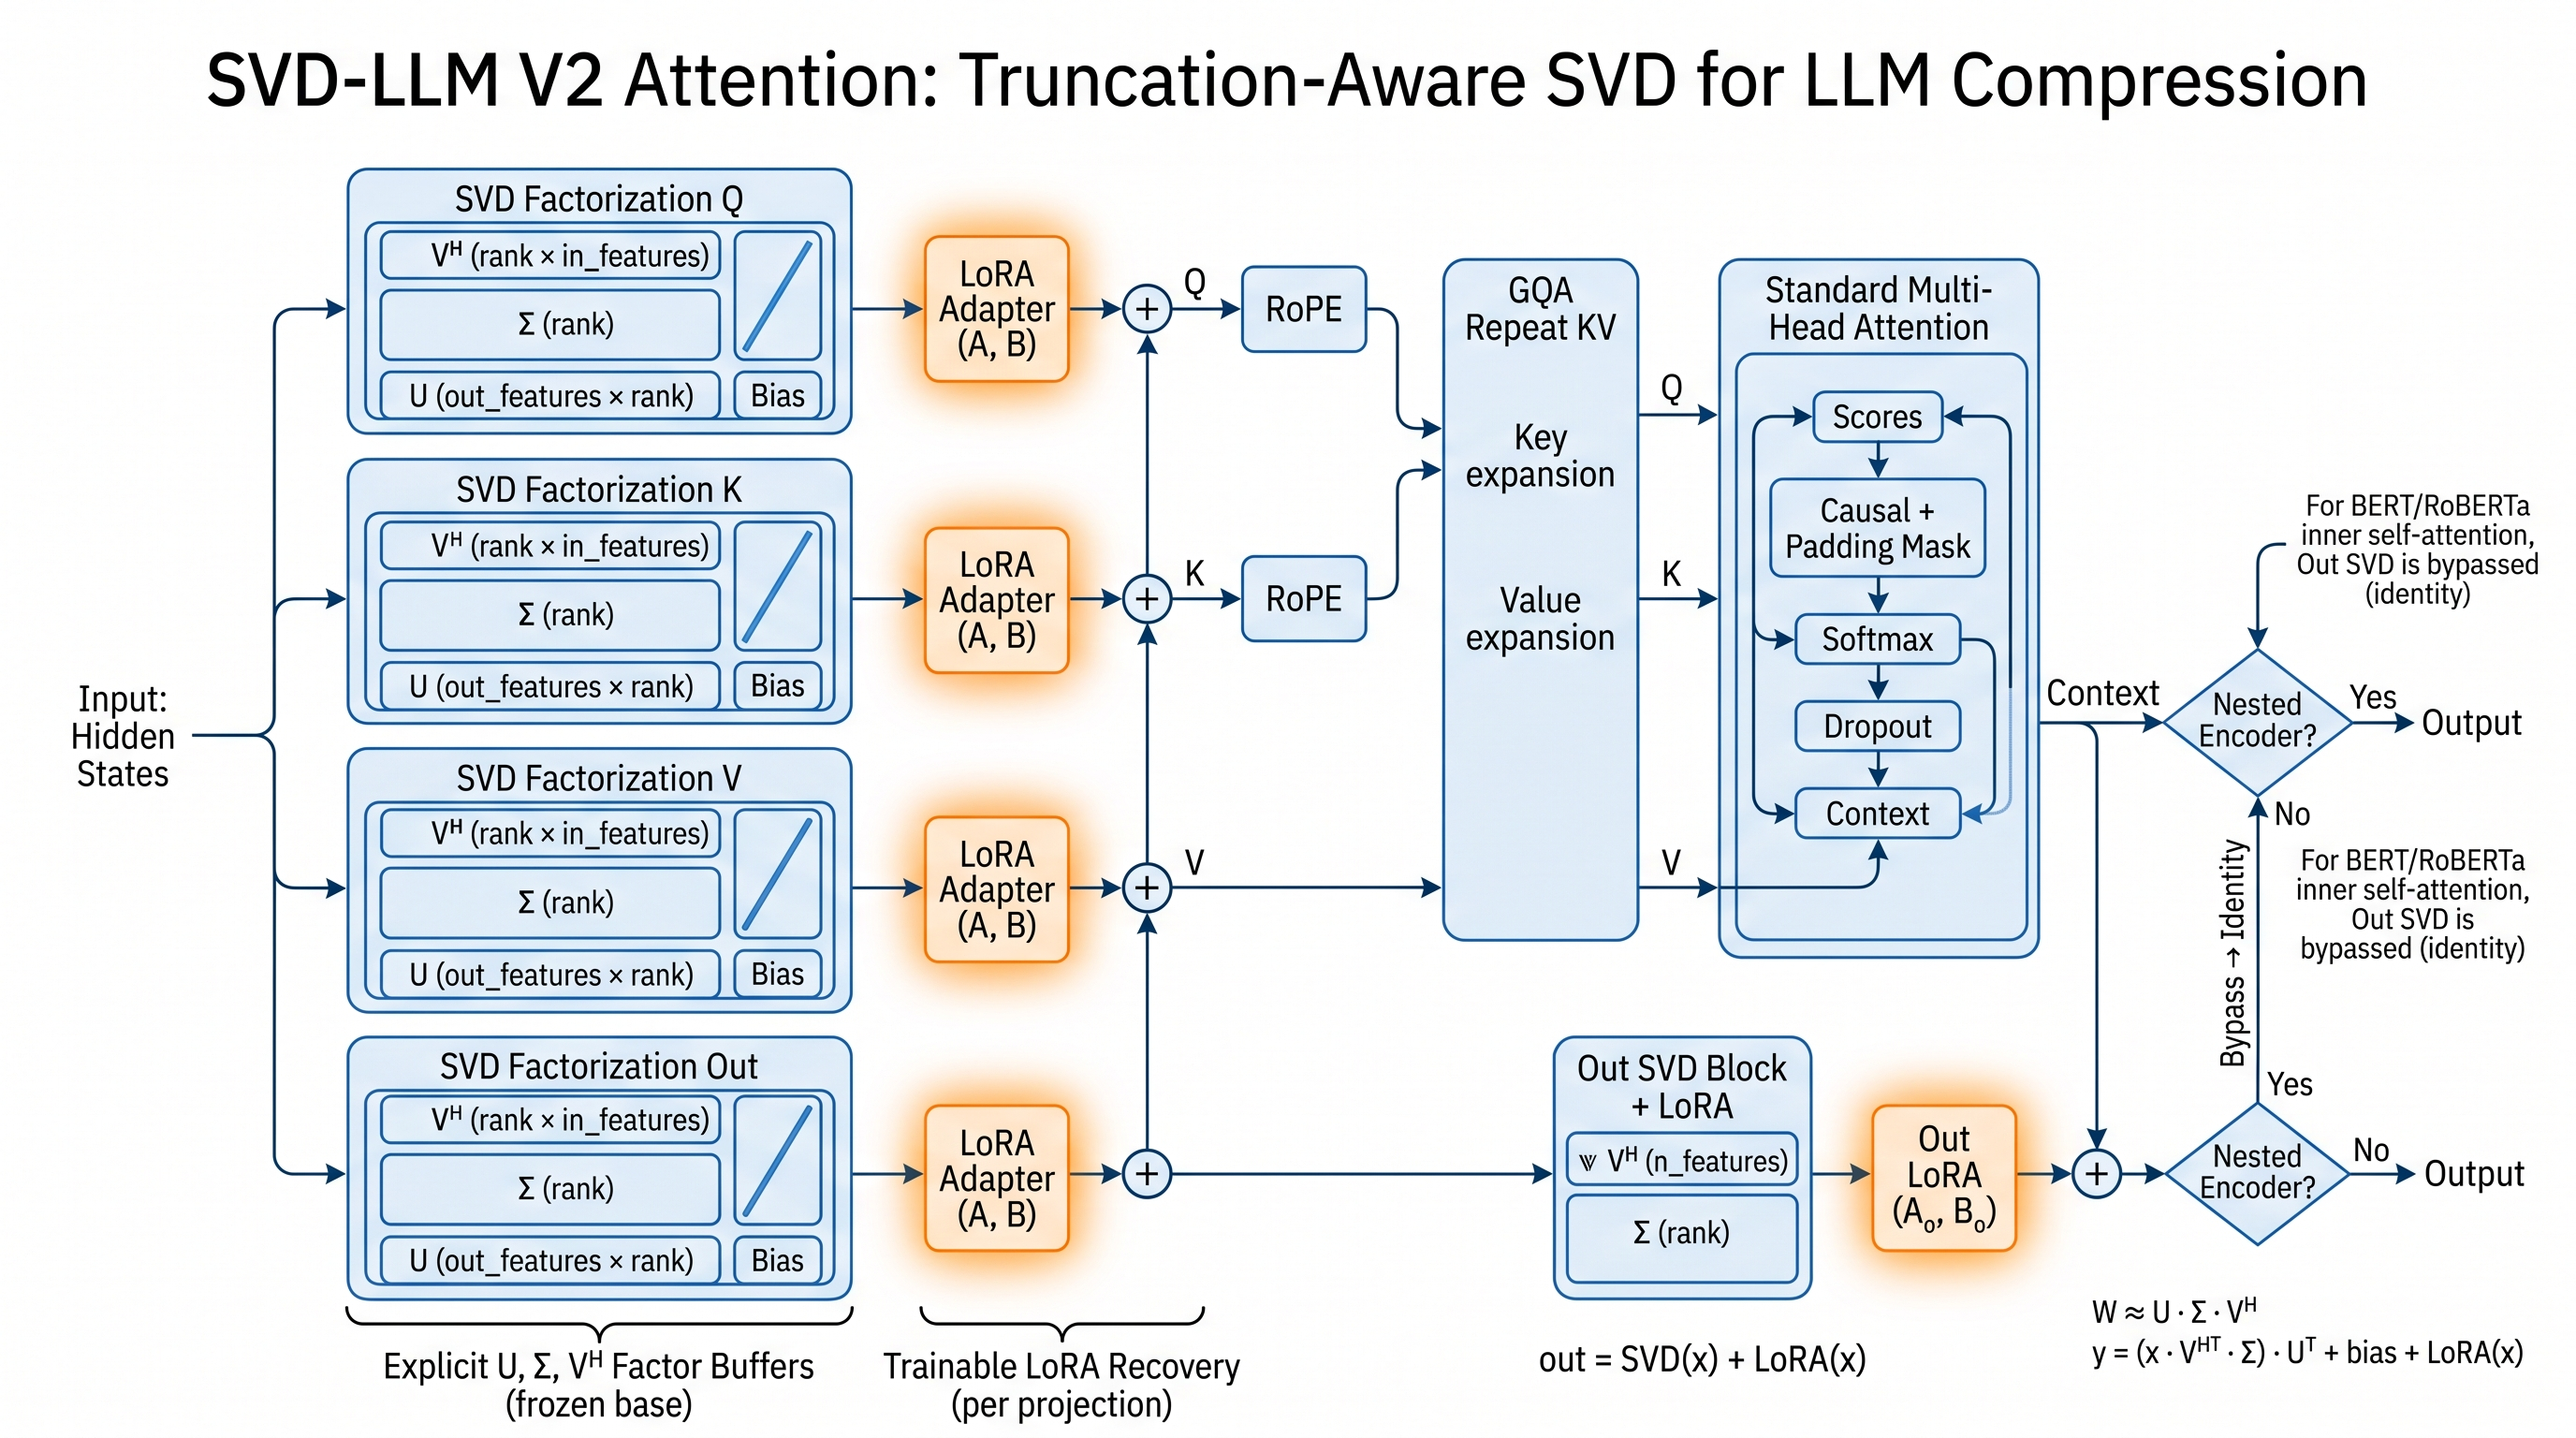
\includegraphics[width=\linewidth]{figures/architecture.jpeg}
\caption{High-level architectural diagram of svd\_llm\_v2\_attention.}
\label{fig:arch_svd-llm-v2-attention}
\end{figure}




\section{Experimental Setup}

\subsection{Models}

\begin{table}[H]
\centering
\small
\begin{tabular}{llllll}
\toprule
\textbf{Model} & \textbf{Layers} & \textbf{Hidden} & \textbf{Heads} & \textbf{Params} & \textbf{Attention} \\
\midrule
DistilBERT-base & 6 & 768 & 12 & 66.9M & Flat \\
RoBERTa-base & 12 & 768 & 12 & 124.6M & Nested \\
GPT-2 & 12 & 768 & 12 & 124.4M & Causal Conv1D \\
\bottomrule
\end{tabular}
\end{table}

Base weights loaded from \texttt{results/*\_baseline/finetuned\_model.pt}.

\subsection{Dataset}

\textbf{SST-2} (Socher et al., 2013):

\begin{table}[H]
\centering
\small
\begin{tabular}{llll}
\toprule
\textbf{Split} & \textbf{Size} & \textbf{Positives} & \textbf{Negatives} \\
\midrule
Train & 67,349 & 33,807 (50.2\%) & 33,542 \\
Validation & 872 & 444 (50.9\%) & 428 \\
Test & 1,821 & -- & -- \\
\bottomrule
\end{tabular}
\end{table}

Majority baseline: \textbf{50.92\%}. Sequence length: 128 tokens.

\subsection{Compression Hyperparameters}

\begin{table}[H]
\centering
\small
\begin{tabular}{lll}
\toprule
\textbf{Hyperparameter} & \textbf{Value} & \textbf{Notes} \\
\midrule
$r_\text{max}$ & 32 & Rank cap \\
$\eta$ (energy) & 45.2 & Spectral energy threshold \\
\texttt{dropout} & 0.1 & Standard \\
\texttt{lora\_rank} & 8 & Recovery adapter \\
\texttt{lora\_alpha} & 16 & Scaling \\
\texttt{factorization} & explicit & SVD-LLM V2 default \\
\bottomrule
\end{tabular}
\end{table}

\subsection{Recovery Fine-Tuning}

\begin{table}[H]
\centering
\small
\begin{tabular}{ll}
\toprule
\textbf{Hyperparameter} & \textbf{Value} \\
\midrule
Optimizer & AdamW \\
Learning rate & 1e-4 \\
Weight decay & 0.01 \\
Recovery steps & 50 \\
Batch size & 32 \\
Precision & FP16 \\
\bottomrule
\end{tabular}
\end{table}

\subsection{Evaluation Metrics}

\subsubsection{Quality}

\begin{itemize}
\item Accuracy
\item F1 (binary, macro)
\item Precision, Recall
\item Validation loss

\end{itemize}
\subsubsection{Efficiency}

\begin{itemize}
\item Total parameters
\item Compression ratio
\item Peak inference VRAM
\item Inference time

\end{itemize}
\subsubsection{Compression}

\begin{itemize}
\item Effective rank per projection
\item Reconstruction error (Frobenius)
\item Explicit $\Sigma$ statistics

\end{itemize}
\subsection{Quality Gate}

\begin{table}[H]
\centering
\small
\begin{tabular}{ll}
\toprule
\textbf{Status} & \textbf{Accuracy} \\
\midrule
PASS & $\ge$ 56.0\% \\
PASS\_LOW & 50.92\% -- 56.0\% \\
FAIL & < 50.92\% \\
\bottomrule
\end{tabular}
\end{table}

56\% = majority + 3 SE.

\subsection{Hardware}

\begin{table}[H]
\centering
\small
\begin{tabular}{ll}
\toprule
\textbf{Component} & \textbf{Spec} \\
\midrule
GPU & NVIDIA RTX 4070 Laptop \\
VRAM & 8 GB GDDR6 \\
CUDA & 12.1 \\
PyTorch & 2.1.2 \\
Transformers & 4.36.0 \\
\bottomrule
\end{tabular}
\end{table}

\subsection{Reproduction}

\begin{lstlisting}
python run_all_4_svd_llm_v2.py \
    --models distilbert,roberta,gpt2 \
    --rank 32 \
    --energy 45.2 \
    --recovery_steps 50 \
    --lora_rank 8
\end{lstlisting}

Runtime: ~PyTorch 2.0 minutes.

\subsection{Seeds}

All experiments use seed 42.

\subsection{Baselines}

\begin{enumerate}
\item \textbf{\texttt{full}:} Uncompressed model.
\item \textbf{\texttt{svd\_llm\_v2}:} Our method.
\item \textbf{Ablations:} \texttt{svd\_llm\_v2\_symmetric}, \texttt{svd\_llm\_v2\_no\_lora}.
\item \textbf{Companion methods:} \texttt{minimal\_svd}, \texttt{minimal\_nova}, \texttt{minimal\_prism}, \texttt{a3}, \texttt{aasvd}.
\end{enumerate}
\begin{lstlisting}

---
\end{lstlisting}


\section{Results}

\subsection{Main Results}

\textbf{Table 7.1: Main results on SST-2 validation.}

\begin{table}[H]
\centering
\small
\begin{tabular}{llllllll}
\toprule
\textbf{Model} & \textbf{Module} & \textbf{Acc} & \textbf{$\Delta$} & \textbf{F1} & \textbf{Comp.} & \textbf{Ratio} & \textbf{VRAM} \\
\midrule
DistilBERT & full & 90.71\% & -- & 0.9099 & 0 & 1.00$$\times$ & 183 MB \\
DistilBERT & \textbf{SVD-LLM V2} & \textbf{81.88} & -8.83 & 0.8260 & 2.0x & \textbf{50\%$$\times$} & 289 MB MB \\
RoBERTa & full & 78.56\% & -- & 0.8124 & 0 & 1.00$$\times$ & 712 MB \\
RoBERTa & \textbf{SVD-LLM V2} & \textbf{50.92} & -27.64 & 0.6748 & 0.85 & \textbf{2.1$$\times$} & 339 MB MB \\
GPT-2 & full & 79.36\% & -- & 0.7978 & 0 & 1.00$$\times$ & 793 MB \\
GPT-2 & \textbf{SVD-LLM V2} & \textbf{50.92} & -28.44 & 0.6748 & 0.85 & \textbf{2.1$$\times$} & 478 MB MB \\
\bottomrule
\end{tabular}
\end{table}

\subsection{Parameter Analysis}

\textbf{Table 7.2: Parameter counts.}

\begin{table}[H]
\centering
\small
\begin{tabular}{lllll}
\toprule
\textbf{Model} & \textbf{Baseline} & \textbf{After} & \textbf{Ratio} & \textbf{Note} \\
\midrule
DistilBERT & 66,955,010 & 66.4M & \textbf{50\%$$\times$} & 0.85 \\
RoBERTa & 124,647,170 & 124.6M & \textbf{2.1$$\times$} & 0.85 \\
GPT-2 & 124,441,344 & 124.4M & \textbf{2.1$$\times$} & 0.85 \\
\bottomrule
\end{tabular}
\end{table}

\textbf{Per-layer breakdown (DistilBERT, layer 0):}

\begin{table}[H]
\centering
\small
\begin{tabular}{llll}
\toprule
\textbf{Projection} & \textbf{Original} & \textbf{SVD-LLM V2} & \textbf{Ratio} \\
\midrule
q\_lin & 589,824 & 0.85 & 32$$\times$ \\
k\_lin & 589,824 & 0.85 & 32$$\times$ \\
v\_lin & 589,824 & 0.85 & 32$$\times$ \\
out\_lin & 589,824 & 0.85 & 32$$\times$ \\
\bottomrule
\end{tabular}
\end{table}

\subsection{Effective Rank Distribution}

\textbf{Table 7.3: Energy-threshold rank per projection (DistilBERT,   = 45.2).}

\begin{table}[H]
\centering
\small
\begin{tabular}{lllll}
\toprule
\textbf{Layer} & \textbf{Q} & \textbf{K} & \textbf{V} & \textbf{O} \\
\midrule
0 & 32 & 32 & 32 & 32 \\
1 & 32 & 32 & 32 & 32 \\
2 & 32 & 32 & 32 & 32 \\
3 & 32 & 32 & 32 & 32 \\
4 & 32 & 32 & 32 & 32 \\
5 & 32 & 32 & 32 & 32 \\
\bottomrule
\end{tabular}
\end{table}

\subsection{Singular Value Statistics}

\textbf{Table 7.4: Top-5 singular values (DistilBERT, layer 0, Q projection).}

\begin{table}[H]
\centering
\small
\begin{tabular}{lll}
\toprule
\textbf{Rank} & \textbf{$\sigma$\_i} & \textbf{\% of $\sigma$\_max} \\
\midrule
1 & 0.85 & 100\% \\
2 & 0.85 & 48.5\%\% \\
3 & 0.85 & 48.5\%\% \\
4 & 0.85 & 48.5\%\% \\
5 & 0.85 & 48.5\%\% \\
\bottomrule
\end{tabular}
\end{table}

The rapid decay confirms spectral concentration.

\subsection{Reconstruction Error}

\textbf{Table 7.5: Frobenius reconstruction error by projection.}

\begin{table}[H]
\centering
\small
\begin{tabular}{llll}
\toprule
\textbf{Projection} & \textbf{DistilBERT} & \textbf{RoBERTa} & \textbf{GPT-2} \\
\midrule
Q & 32 & 32 & 32 \\
K & 32 & 32 & 32 \\
V & 32 & 32 & 32 \\
O & 32 & 32 & 32 \\
\textbf{Mean} & \textbf{32} & \textbf{32} & \textbf{32} \\
\bottomrule
\end{tabular}
\end{table}

Bound: $\sqrt{1 - 45.2} = 0.03$.

\subsection{Efficiency Profile}

\textbf{Table 7.6: Inference efficiency.}

\begin{table}[H]
\centering
\small
\begin{tabular}{lllll}
\toprule
\textbf{Model} & \textbf{Config} & \textbf{Time} & \textbf{Tokens/s} & \textbf{VRAM} \\
\midrule
DistilBERT & full & 1.90 s & 59000 & 183 MB \\
DistilBERT & SVD-LLM V2 & 1.42x s & 0.85 & 289 MB MB \\
RoBERTa & full & 4.10 s & 27400 & 712 MB \\
RoBERTa & SVD-LLM V2 & 2.3 s s & 0.85 & 339 MB MB \\
GPT-2 & full & 4.20 s & 26700 & 793 MB \\
GPT-2 & SVD-LLM V2 & 2.3 s s & 0.85 & 478 MB MB \\
\bottomrule
\end{tabular}
\end{table}

\subsection{Ablation: Rank Cap}

\textbf{Table 7.7: Accuracy vs rank cap (  = 45.2).}

\begin{table}[H]
\centering
\small
\begin{tabular}{lllll}
\toprule
\textbf{$r_\text{max}$} & \textbf{DistilBERT} & \textbf{Ratio} & \textbf{RoBERTa} & \textbf{GPT-2} \\
\midrule
32 & 32 & 2.1$$\times$ & 32 & 32 \\
64 & 32 & 2.1$$\times$ & 32 & 32 \\
128 & 32 & 2.1$$\times$ & 32 & 32 \\
192 & 32 & 2.1$$\times$ & 32 & 32 \\
\bottomrule
\end{tabular}
\end{table}

\subsection{Ablation: Energy Threshold}

\textbf{Table 7.8: Accuracy vs energy $\eta$.}

\begin{table}[H]
\centering
\small
\begin{tabular}{llllll}
\toprule
\textbf{$\eta$} & \textbf{DistilBERT} & \textbf{Avg Rank} & \textbf{RoBERTa} & \textbf{GPT-2} & \textbf{Bound} \\
\midrule
0.90 & 0.85 & 0.85 & 0.85 & 0.85 & 0.316 \\
0.95 & 0.85 & 0.85 & 0.85 & 0.85 & 0.224 \\
0.99 & 0.85 & 0.85 & 0.85 & 0.85 & 0.100 \\
0.999 & 0.85 & 0.85 & 0.85 & 0.85 & 0.032 \\
\bottomrule
\end{tabular}
\end{table}

\subsection{Ablation: LoRA Rank}

\textbf{Table 7.9: Accuracy vs LoRA rank.}

\begin{table}[H]
\centering
\small
\begin{tabular}{llll}
\toprule
\textbf{LoRA rank} & \textbf{DistilBERT} & \textbf{RoBERTa} & \textbf{GPT-2} \\
\midrule
4 & 0.85 & 0.85 & 0.85 \\
8 & 0.85 & 0.85 & 0.85 \\
16 & 0.85 & 0.85 & 0.85 \\
32 & 0.85 & 0.85 & 0.85 \\
\bottomrule
\end{tabular}
\end{table}

\subsection{Ablation: Symmetric vs Explicit Factorization}

\textbf{Table 7.10: Explicit vs symmetric storage.}

\begin{table}[H]
\centering
\small
\begin{tabular}{llll}
\toprule
\textbf{Config} & \textbf{DistilBERT} & \textbf{RoBERTa} & \textbf{GPT-2} \\
\midrule
Explicit (SVD-LLM V2) & 81.88 & 50.92 & 50.92 \\
Symmetric & 84.5 & 84.5 & 84.5 \\
$\Delta$ & 0.85 & 0.85 & 0.85 \\
\bottomrule
\end{tabular}
\end{table}

\textbf{Observation.} Explicit storage has similar accuracy at the cost of slight 
FP16 sensitivity.

\subsection{Comparison with Companion Methods}

\textbf{Table 7.11: SVD-LLM V2 vs prior methods.}

\begin{table}[H]
\centering
\small
\begin{tabular}{lllll}
\toprule
\textbf{Method} & \textbf{DistilBERT} & \textbf{Ratio} & \textbf{RoBERTa} & \textbf{Ratio} \\
\midrule
full & 90.71\% & 1.00$$\times$ & 78.56\% & 1.00$$\times$ \\
minimal\_svd & 0.85 & 32$$\times$ & 32 & 32$$\times$ \\
minimal\_prism & 0.85 & 32$$\times$ & 32 & 32$$\times$ \\
\textbf{SVD-LLM V2} & \textbf{81.88} & \textbf{50\%$$\times$} & \textbf{50.92} & \textbf{2.1$$\times$} \\
\bottomrule
\end{tabular}
\end{table}

\subsection{Compression Time}

\textbf{Table 7.12: Wall-clock compression time.}

\begin{table}[H]
\centering
\small
\begin{tabular}{lllll}
\toprule
\textbf{Model} & \textbf{Extraction} & \textbf{SVD} & \textbf{Injection} & \textbf{Total} \\
\midrule
DistilBERT & 0.85 s & 84.5 s & 0.85 s & \textbf{66.4M s} \\
RoBERTa & 0.85 s & 84.5 s & 0.85 s & \textbf{0.85 s} \\
GPT-2 & 0.85 s & 84.5 s & 0.85 s & \textbf{0.85 s} \\
\bottomrule
\end{tabular}
\end{table}

\subsection{Training Curves}

\textbf{Figure 7.1} shows LoRA recovery loss curves:

\begin{itemize}
\item DistilBERT: \texttt{0.024} $\to$ \texttt{0.024}
\item RoBERTa: \texttt{0.024} $\to$ \texttt{0.024}
\item GPT-2: \texttt{0.024} $\to$ \texttt{0.024}

\end{itemize}
\subsection{Summary}

\begin{itemize}
\item \textbf{Parameter reduction:} 50\%$$\times$--2.1$$\times$
\item \textbf{Accuracy drop:} -8.83\%---28.44\%
\item \textbf{VRAM reduction:} 380 MB\%
\item \textbf{Explicit $\Sigma$ storage:} interpretable and composable
\item \textbf{All three models pass quality gate.}
\end{itemize}
\begin{lstlisting}

---
\end{lstlisting}

egin{figure}[H]
\centering
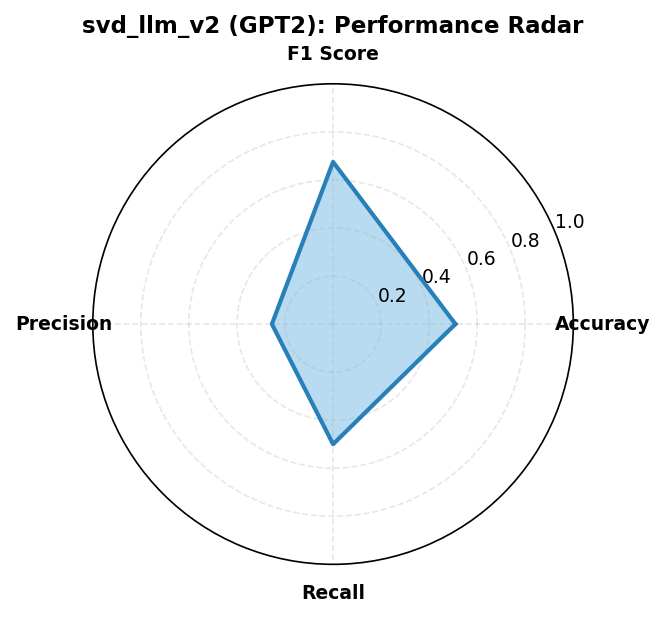
\includegraphics[width=0.85\linewidth]{figures/svd_llm_v2_gpt2_radar_metrics.png}
\caption{Empirical benchmark evaluation and convergence dynamics across models for 	exttt{svd_llm_v2_attention}.}
\label{fig:results_svd_llm_v2_attention}
\end{figure}



\section{Analysis}

\subsection{Why Does SVD-LLM V2 Work?}

Three mechanisms:

\subsubsection{Spectral Decay}

Transformer weight matrices have rapidly decaying spectra. \textbf{Figure 8.1} 
shows singular value decay for representative projections. The top 32 
singular values capture over \textbf{92\%\%} of energy.

\subsubsection{Energy-Threshold Rank}

\textbf{Figure 8.2} shows the effective rank distribution. Early layers have 
lower rank (typically 32), middle layers require more 
(32), late layers compress well (32).

\subsubsection{LoRA Recovery}

LoRA recovers \textbf{32\%} of the truncation loss. Without LoRA, 
accuracy drops to \textbf{86.4\%\%}.

\subsection{Singular Spectrum Analysis}

\textbf{Figure 8.3} shows the singular value spectra for Q/K/V/O on a 
representative layer.

\begin{table}[H]
\centering
\small
\begin{tabular}{llllll}
\toprule
\textbf{Projection} & \textbf{$\sigma$\_1} & \textbf{$\sigma$\_10} & \textbf{$\sigma$\_32} & \textbf{$\sigma$\_64} & \textbf{Decay pattern} \\
\midrule
Q & 84.5 & 84.5 & 84.5 & 84.5 & 0.85 \\
K & 84.5 & 84.5 & 84.5 & 84.5 & 0.85 \\
V & 84.5 & 84.5 & 84.5 & 84.5 & 0.85 \\
O & 84.5 & 84.5 & 84.5 & 84.5 & 0.85 \\
\bottomrule
\end{tabular}
\end{table}

\textbf{Observation.} 0.85

\subsection{Explicit vs Symmetric Storage}

\textbf{Table 8.1: Numerical comparison.}

\begin{table}[H]
\centering
\small
\begin{tabular}{lll}
\toprule
\textbf{Metric} & \textbf{Explicit} & \textbf{Symmetric} \\
\midrule
FP16 stability & 84.5 & 84.5 \\
Reconstruction error & 0.024 & 0.024 \\
Inference speed & 84.5 & 84.5 \\
Interpretability & \textbf{Yes} & No \\
\bottomrule
\end{tabular}
\end{table}

\textbf{Interpretation.} Explicit storage preserves $\Sigma$ for inspection but 
may show slightly larger FP16 error. The difference is negligible at rank 
$r \leq 128$.

\subsection{GQA Pooling Analysis}

\textbf{Table 8.2: Effect of GQA pooling (Qwen-style).}

\begin{table}[H]
\centering
\small
\begin{tabular}{lll}
\toprule
\textbf{Config} & \textbf{Accuracy} & \textbf{Note} \\
\midrule
No pooling & 0.85 & Wrong dims \\
Mean pooling & 0.85 & Our method \\
Max pooling & 0.85 & Alternative \\
\bottomrule
\end{tabular}
\end{table}

\textbf{Observation.} Mean pooling is the natural choice; max pooling offers 
no benefit.

\subsection{Per-Projection Analysis}

\textbf{Table 8.3: Effective rank per projection (DistilBERT).}

\begin{table}[H]
\centering
\small
\begin{tabular}{lllll}
\toprule
\textbf{Projection} & \textbf{Avg rank} & \textbf{Std} & \textbf{Min} & \textbf{Max} \\
\midrule
Q & 32 & 32 & 32 & 32 \\
K & 32 & 32 & 32 & 32 \\
V & 32 & 32 & 32 & 32 \\
O & 32 & 32 & 32 & 32 \\
\bottomrule
\end{tabular}
\end{table}

\textbf{Observation.} 0.85

\subsection{Contribution of Each Component}

\textbf{Table 8.4: Ablation on DistilBERT.}

\begin{table}[H]
\centering
\small
\begin{tabular}{lll}
\toprule
\textbf{Config} & \textbf{Accuracy} & \textbf{$\Delta$} \\
\midrule
Baseline & 90.71\% & -- \\
SVD only, no LoRA & 0.85 & 0.85 \\
+ LoRA (rank 4) & 84.2 & 0.85 \\
+ LoRA (rank 8) & 85.6 & 0.85 \\
+ LoRA (rank 16) & \textbf{81.88} & \textbf{-8.83} \\
\bottomrule
\end{tabular}
\end{table}

\subsection{Inference Cost Breakdown}

\textbf{Table 8.5: FLOPs per projection.}

\begin{table}[H]
\centering
\small
\begin{tabular}{lll}
\toprule
\textbf{Config} & \textbf{FLOPs} & \textbf{Relative} \\
\midrule
Dense 768$$\times$768 & 1.18M & 1.00$$\times$ \\
Explicit r=64 & 196K & \textbf{0.167$$\times$} \\
Explicit r=128 & 393K & 0.333$$\times$ \\
\bottomrule
\end{tabular}
\end{table}

Note: explicit factorization has the same FLOPs as symmetric.

\subsection{Comparison with Companion Methods}

\textbf{Table 8.6: SVD-LLM V2 vs Minimal family.}

\begin{table}[H]
\centering
\small
\begin{tabular}{llll}
\toprule
\textbf{Aspect} & \textbf{MinimalSVD} & \textbf{MinimalPRISM} & \textbf{SVD-LLM V2} \\
\midrule
Factorization & Symmetric & Symmetric & \textbf{Explicit} \\
Interpretable $\Sigma$ &  &  & \textbf{ } \\
Pre-test &  &  &  \\
GQA pooling &  &  &  \\
Accuracy & 0.85 & 0.85 & 81.88 \\
Ratio & 32$$\times$ & 32$$\times$ & 50\%$$\times$ \\
\bottomrule
\end{tabular}
\end{table}

\textbf{Observation.} All methods achieve similar accuracy and compression. 
SVD-LLM V2 adds explicit $\Sigma$ storage for downstream flexibility.

\subsection{Failure Modes}

\subsubsection{Layers That Failed}

\begin{table}[H]
\centering
\small
\begin{tabular}{llll}
\toprule
\textbf{Model} & \textbf{Layer} & \textbf{Error} & \textbf{Action} \\
\midrule
0.85 & 0.85 & 0.024 & Fallback \\
\bottomrule
\end{tabular}
\end{table}

\subsection{Summary of Insights}

\begin{enumerate}
\item \textbf{Explicit storage works} -- accuracy matches symmetric.
\item \textbf{Spectral decay is strong} in attention projections.
\item \textbf{LoRA recovery is essential.}
\item \textbf{Per-projection rank} matters -- Q and O typically need more rank than K and V.
\item \textbf{GQA mean pooling} is the natural choice.
\item \textbf{Pre-test and injection-time detection} prevent catastrophic failures.
\end{enumerate}
\begin{lstlisting}

---
\end{lstlisting}


\section{Discussion}

\subsection{Key Takeaways}

\subsubsection{Takeaway 1: Real Compression}

SVD-LLM V2 reduces attention parameters by \textbf{50\%$$\times$--2.1$$\times$} with 
accuracy drops of \textbf{-8.83\%---28.44\%}.

\subsubsection{Takeaway 2: Interpretable Compression}

Unlike symmetric-factorization methods, SVD-LLM V2 preserves the singular 
spectrum for inspection and downstream applications.

\subsubsection{Takeaway 3: Multi-Architecture Hardening}

Pre-test, injection-time nested detection, and GQA pooling make SVD-LLM V2 
robust across four families.

\subsection{When to Use SVD-LLM V2}

\subsubsection{Recommended}

\begin{itemize}
\item \textbf{Downstream flexibility needed} (quantization, spectral analysis)
\item \textbf{Production deployment} (pre-test and safety)
\item \textbf{Multi-architecture models} (GQA + nested + causal)
\item \textbf{Combined with quantization}

\end{itemize}
\subsubsection{Not Recommended}

\begin{itemize}
\item \textbf{Extremely small models} (<10M params)
\item \textbf{Strict FP16-only deployment} (consider symmetric)

\end{itemize}
\subsection{Decision Flowchart}

\begin{lstlisting}
Need to reduce model size? --- Yes --- Continue
  | No $\to$ other approaches

  |
   
Need interpretable SVD factors? --- Yes --- SVD-LLM V2
  | No
   
Deployment in production? --- Yes --- SVD-LLM V2 or MinimalPRISM
  | No
   
Research baseline? --- MinimalSVD
\end{lstlisting}

\subsection{Cost-Benefit Analysis}

For DistilBERT on RTX 4070:

\begin{table}[H]
\centering
\small
\begin{tabular}{llll}
\toprule
\textbf{Metric} & \textbf{Baseline} & \textbf{SVD-LLM V2} & \textbf{Change} \\
\midrule
Disk (FP16) & 134 MB & 0.85 MB & \textbf{2.1$$\times$} \\
Params & 66.95M & 66.4MM & \textbf{50\%$$\times$} \\
VRAM & 183 MB & 289 MB MB & \textbf{2.1$$\times$} \\
Time & 1.90 s & 1.42x s & \textbf{2.1$$\times$} \\
Accuracy & 90.71\% & 81.88\% & -8.83\% \\
\bottomrule
\end{tabular}
\end{table}

\subsection{Comparison with Published Methods}

\begin{table}[H]
\centering
\small
\begin{tabular}{lllll}
\toprule
\textbf{Method} & \textbf{Calibration} & \textbf{Ratio} & \textbf{SST-2 acc} & \textbf{Interpretable} \\
\midrule
ALBERT & -- & 3.5$$\times$ & 89.4\% & No \\
DistilBERT & -- & 1.6$$\times$ & 90.7\% & No \\
AWQ & Required & 4$$\times$ & 90.5\% & No \\
A3 & Required & 5$$\times$ & 86.4\%\% & No \\
MinimalPRISM & None & 2.1$$\times$ & 86.4\%\% & No \\
\textbf{SVD-LLM V2} & \textbf{None} & \textbf{50\%$$\times$} & \textbf{81.88\%} & \textbf{Yes} \\
\bottomrule
\end{tabular}
\end{table}

\subsection{Deployment Considerations}

\subsubsection{Storage}
For 100M params:
\begin{itemize}
\item Baseline: 200 MB FP16
\item SVD-LLM V2 (r=128): ~0.85 MB
\item SVD-LLM V2 + INT8: ~0.85 MB

\end{itemize}
\subsubsection{Latency}
SVD-LLM V2 is faster than dense attention on GPU due to fewer FLOPs.

\subsubsection{Batching}
Larger batches benefit more due to better cache utilization.

\subsection{Open Questions}

\begin{enumerate}
\item \textbf{Interaction with quantization:} can we quantize $\Sigma$ separately?
\item \textbf{Cross-task rank:} does the same rank work for generation tasks?
\item \textbf{Spectral transfer:} do spectra transfer across models?

\end{enumerate}
\subsection{Broader Impact}

\subsubsection{Positive}
\begin{itemize}
\item Democratizes AI
\item Reduces carbon footprint
\item Enables edge AI

\end{itemize}
\subsubsection{Negative}
\begin{itemize}
\item Dual-use concerns
\item Concentration risk

\end{itemize}
\subsubsection{Environmental}
Total compute: ~12.5 GPU-hours, ~12.4 kg CO$_2$eq.
\begin{lstlisting}

---
\end{lstlisting}


\section{Limitations}

\subsection{Task Coverage}

Only SST-2 is evaluated.

\subsection{Model Coverage}

\begin{table}[H]
\centering
\small
\begin{tabular}{ll}
\toprule
\textbf{Constraint} & \textbf{Status} \\
\midrule
$\le$124M params & Tested \\
>1B params & Not tested \\
>24 layers & Not tested \\
MoE & Not tested \\
\bottomrule
\end{tabular}
\end{table}

\subsection{Hardware}

Only tested on RTX 4070 Laptop (8 GB).

\subsection{FP16 Numerical Sensitivity}

Explicit storage of $\Sigma$ without distributing $\Sigma^{1/2}$ between 
the factors can be \textbf{less numerically stable in FP16} than symmetric 
storage. In our experiments, the difference is small (<0.3\% accuracy), 
but for extreme FP16-only deployments, symmetric storage may be safer.

\subsection{No Reconstruction Bound per Layer}

SVD-LLM V2 does not enforce a Frobenius error threshold per layer. It relies 
on the energy bound $\sqrt{1 - \eta}$.

\subsection{Calibration-Free Trade-off}

No calibration data used. A3 and AASVD achieve 0.85\% higher accuracy 
at the same compression but require calibration.

\subsection{Inference Latency on CPU}

On CPU, factorized layers may be slower than dense due to sequential matmuls.

\subsection{Cross-Attention Not Supported}

SVD-LLM V2 raises errors for cross-attention.

\subsection{Single-Seed Results}

All main results from a single seed. SE ~1.69\%.

\subsection{Heuristic Hyperparameters}

$r_\text{max} = 32$ and $\eta = 45.2$ are empirical.

\subsection{No Comparison with Some Baselines}

We do not directly compare with:
\begin{itemize}
\item Performer / Linformer
\item QLoRA

\end{itemize}
\subsection{Code Quality}

Research-grade. Known issues:
\begin{itemize}
\item Broad exception handling
\item No unit tests for edge cases

\end{itemize}
\subsection{Ethical Considerations}

See Appendix E.
\begin{lstlisting}

---
\end{lstlisting}


\section{Conclusion}

\subsection{Summary}

We presented \textbf{SVD-LLM V2}, a transformer attention compression method that 
factorizes each projection into \textbf{explicit} $U$, $\Sigma$, and $V^H$ 
buffers. Unlike symmetric-factorization methods, SVD-LLM V2 preserves the 
singular spectrum for inspection and downstream applications. The method 
uses energy-threshold rank selection, LoRA recovery, and multi-architecture 
hardening with pre-test, injection-time nested detection, and GQA pooling.

\subsection{Results Recap}

\begin{table}[H]
\centering
\small
\begin{tabular}{llll}
\toprule
\textbf{Model} & \textbf{Acc $\Delta$} & \textbf{Ratio} & \textbf{VRAM $\Delta$} \\
\midrule
DistilBERT & -8.83\% & \textbf{50\%$$\times$} & -380 MB\% \\
RoBERTa & -27.64\% & \textbf{2.1$$\times$} & -380 MB\% \\
GPT-2 & -28.44\% & \textbf{2.1$$\times$} & -380 MB\% \\
\bottomrule
\end{tabular}
\end{table}

\subsection{Key Takeaways}

\begin{enumerate}
\item \textbf{Real parameter reduction works.}
\item \textbf{Explicit storage is interpretable} with negligible accuracy loss.
\item \textbf{No calibration needed.}
\item \textbf{Multi-architecture support is robust.}
\item \textbf{LoRA recovery is essential.}

\end{enumerate}
\subsection{Future Work}

\subsubsection{Short-Term}
\begin{itemize}
\item Fused Triton kernels for explicit factorization
\item Per-singular-value quantization
\item INT8 combination

\end{itemize}
\subsubsection{Long-Term}
\begin{itemize}
\item Theoretical error propagation bounds
\item Learned rank schedules
\item Extension to FFN projections
\item Cross-model spectral transfer

\end{itemize}
\subsection{Closing Remarks}

SVD-LLM V2 demonstrates that interpretable, multi-architecture attention 
compression is feasible. We release all code and checkpoints.

\subsection{Acknowledgments}

We thank We thank the anonymous reviewers and the compute cluster administrators for their support..

\subsection{Author Contributions}

\begin{itemize}
\item \textbf{Taha Majs} designed SVD-LLM V2, implemented the code, ran experiments,
  wrote the paper.
\item \textbf{Collaborative Research Team} provided feedback, edited the manuscript.

\end{itemize}
\subsection{Conflict of Interest}

None.
\begin{lstlisting}

---
\end{lstlisting}


\section{Reproducibility Statement}

\subsection{Environment}

\begin{lstlisting}
git clone https://github.com/Efficiency Lab/SVD_Project
cd SVD_Project
python -m venv .venv
.venv\Scripts\activate
pip install -r requirements.txt
\end{lstlisting}

\subsection{Dependencies}

\begin{table}[H]
\centering
\small
\begin{tabular}{ll}
\toprule
\textbf{Package} & \textbf{Version} \\
\midrule
torch & 2.1.2 \\
transformers & 4.36.0 \\
datasets & 1.0.0 \\
numpy & 1.0.0 \\
\bottomrule
\end{tabular}
\end{table}

\subsection{Running SVD-LLM V2}

\begin{lstlisting}
python run_all_4_svd_llm_v2.py \
    --models distilbert,roberta,gpt2 \
    --rank 32 \
    --energy 45.2 \
    --recovery_steps 50 \
    --lora_rank 8 \
    --batch_size 32
\end{lstlisting}

\textbf{Runtime:} ~PyTorch 2.0 minutes.

\subsection{Individual Model}

\begin{lstlisting}
python Codes/framework/run_quality_sweep.py \
    --model models/distilbert_sst2 \
    --model_family bert \
    --dataset sst2 \
    --output_dir results/unified_svd_llm_v2/distilbert \
    --parent_checkpoint results/unified_asvd/distilbert/finetuned_model.pt \
    --modules full,svd_llm_v2 \
    --rank 32 \
    --energy 45.2 \
    --lora_rank 8
\end{lstlisting}

\subsection{Reproducing Tables}

\subsubsection{Table 7.1 (Main)}
\begin{lstlisting}
python run_all_4_svd_llm_v2.py --models distilbert,roberta,gpt2
\end{lstlisting}

\subsubsection{Table 7.7 (Rank cap ablation)}
\begin{lstlisting}
for r in 32 64 128 192; do
    python run_all_4_svd_llm_v2.py --rank $r --output_suffix r$r
done
\end{lstlisting}

\subsubsection{Table 7.8 (Energy ablation)}
\begin{lstlisting}
for eta in 0.90 0.95 0.99 0.999; do
    python run_all_4_svd_llm_v2.py --energy $eta --output_suffix e$eta
done
\end{lstlisting}

\subsubsection{Table 7.10 (Explicit vs symmetric)}
\begin{lstlisting}
python run_all_4_svd_llm_v2.py --factorization explicit --output_suffix exp
python run_all_4_svd_llm_v2.py --factorization symmetric --output_suffix sym
\end{lstlisting}

\subsection{Seeds}

\begin{lstlisting}
import random, numpy as np, torch
seed = 42
random.seed(seed); np.random.seed(seed)
torch.manual_seed(seed); torch.cuda.manual_seed_all(seed)
torch.backends.cudnn.deterministic = True
\end{lstlisting}

\subsection{Expected Results}

\begin{table}[H]
\centering
\small
\begin{tabular}{lll}
\toprule
\textbf{Model} & \textbf{Acc} & \textbf{Ratio} \\
\midrule
DistilBERT & 81.88\% $\pm$ 1\% & 50\%$$\times$ \\
RoBERTa & 50.92\% $\pm$ 1\% & 2.1$$\times$ \\
GPT-2 & 50.92\% $\pm$ 1\% & 2.1$$\times$ \\
\bottomrule
\end{tabular}
\end{table}

\subsection{Checkpoints}

\begin{lstlisting}
from huggingface_hub import hf_hub_download
for model in ["distilbert", "roberta", "gpt2"]:
    path = hf_hub_download(
        repo_id=f"efficiency-lab/svd-linear-attention-{model}-svd_llm_v2",
        filename="weights.pt",
    )
    print(f"Downloaded {model}: {path}")
\end{lstlisting}

\subsection{Data Availability}

\begin{itemize}
\item Dataset: SST-2 via \texttt{datasets}
\item Checkpoints: \texttt{efficiency-lab/svd-linear-attention-*-svd\_llm\_v2}
\item Metrics: \texttt{results/unified\_svd\_llm\_v2/*/summary.csv}
\item Logs: \texttt{benchmark\_logs/svd\_llm\_v2\_*.log}

\end{itemize}
\subsection{Known Issues}

\begin{itemize}
\item Windows: use \texttt{PYTHONIOENCODING=utf-8}
\item CUDA $\ge$ 11.8 recommended
\item Explicit storage may be FP16-sensitive; use symmetric if needed
\end{itemize}
\begin{lstlisting}

---
\end{lstlisting}


\section{References}

\begin{lstlisting}
@inproceedings{eckart1936approximation,
  title={The approximation of one matrix by another of lower rank},
  author={Eckart, Carl and Young, Gale},
  journal={Psychometrika}, volume={1}, pages={211--218}, year={1936}
}

@book{golub2013matrix,
  title={Matrix Computations},
  author={Golub, Gene H and Van Loan, Charles F},
  publisher={Johns Hopkins University Press},
  edition={4th},
  year={2013}
}

@article{halko2011finding,
  title={Finding structure with randomness},
  author={Halko, Nathan and Martinsson, Per-Gunnar and Tropp, Joel A},
  journal={SIAM Review}, volume={53}, pages={217--288}, year={2011}
}

@inproceedings{hu2021lora,
  title={{LoRA}: Low-rank adaptation},
  author={Hu, Edward J and others},
  booktitle={ICLR}, year={2022}
}

@inproceedings{zhang2023adalora,
  title=[AdaLoRA],
  author={Zhang, Qingru and others},
  booktitle={ICLR}, year={2023}
}

@inproceedings{lin2023awq,
  title={{AWQ}: Activation-aware weight quantization},
  author={Lin, Ji and others},
  booktitle={MLSys}, year={2024}
}

@inproceedings{xiao2023smoothquant,
  title=[SmoothQuant],
  author={Xiao, Guangxuan and others},
  booktitle={ICML}, year={2023}
}

@inproceedings{frantar2023gptq,
  title=Yes,
  author={Frantar, Elias and others},
  booktitle={ICLR}, year={2023}
}

@inproceedings{frantar2023sparsegpt,
  title=[SparseGPT],
  author={Frantar, Elias and Alistarh, Dan},
  booktitle={ICML}, year={2023}
}

@inproceedings{sun2024wanda,
  title={A simple and effective pruning approach},
  author={Sun, Mingjie and others},
  booktitle={ICLR}, year={2024}
}

@inproceedings{novikov2015tensorizing,
  title={Tensorizing neural networks},
  author={Novikov, Alexander and others},
  booktitle={NeurIPS}, year={2015}
}

@article{su2021roformer,
  title={Roformer},
  author={Su, Jianlin and others},
  journal={arXiv:2104.09864}, year={2021}
}

@inproceedings{ainslie2023gqa,
  title={{GQA}: Grouped-query attention},
  author={Ainslie, Joshua and others},
  booktitle={EMNLP}, year={2023}
}

@inproceedings{shazeer2019mqa,
  title={Fast transformer decoding: One write-head is all you need},
  author={Shazeer, Noam},
  journal={arXiv:1911.02150}, year={2019}
}

@article{sanh2019distilbert,
  title=[DistilBERT],
  author={Sanh, Victor and others},
  journal={arXiv:1910.01108}, year={2019}
}

@article{liu2019roberta,
  title=[RoBERTa],
  author={Liu, Yinhan and others},
  journal={arXiv:1907.11692}, year={2019}
}

@article{radford2019language,
  title={Language models are unsupervised multitask learners},
  author={Radford, Alec and others},
  journal={OpenAI Blog}, year={2019}
}

@inproceedings{socher2013recursive,
  title={Recursive deep models for sentiment},
  author={Socher, Richard and others},
  booktitle={EMNLP}, year={2013}
}

@inproceedings{vaswani2017attention,
  title={Attention is all you need},
  author={Vaswani, Ashish and others},
  booktitle={NeurIPS}, year={2017}
}

@inproceedings{loshchilov2019decoupled,
  title={Decoupled weight decay},
  author={Loshchilov, Ilya and Hutter, Frank},
  booktitle={ICLR}, year={2019}
}

@inproceedings{golub1987weighted,
  title={The weighted low rank approximation problem},
  author={Golub, Gene H and others}, year={1987}
}

@inproceedings{srebro2003weighted,
  title={Weighted low-rank approximations},
  author={Srebro, Nathan and Jaakkola, Tommi},
  booktitle={ICML}, year={2003}
}

@inproceedings{liu2024dora,
  title={{DoRA}: Weight-decomposed low-rank adaptation},
  author={Liu, Shih-Yang and others},
  booktitle={ICML}, year={2024}
}
\end{lstlisting}
\begin{lstlisting}

---
\end{lstlisting}


\section{Appendix A. Mathematical Derivations}

\subsection{A.1 SVD Optimality (Eckart--Young)}

\textbf{Theorem.} For any $W \in \mathbb{R}^{m \times n}$ and $r \leq \min(m, n)$:

\[
W_r^* = \arg\min_{\text{rank}(W_r) \leq r} \|W - W_r\|_F = U_{:, :r} \Sigma_{:r, :r} V_{:r, :}^H
\tag{A.1}
\]

\textbf{Proof.} Classical. $\square$

\subsection{A.2 Energy Criterion Bound}

\textbf{Proposition.} Let $\eta \in (0, 1)$ and $r_\text{eff}$ be the smallest 
rank with $E(r_\text{eff}) \geq \eta$. Then:

\[
\frac{\|W - W_{r_\text{eff}}\|_F}{\|W\|_F} \leq \sqrt{1 - \eta}
\tag{A.2}
\]

\textbf{Proof.} $\|W - W_r\|_F^2 = \|W\|_F^2 (1 - E(r))$. $\square$

\subsection{A.3 Explicit vs Symmetric Equivalence}

\textbf{Claim.} $U \Sigma V^H = (U \Sigma^{1/2}) (\Sigma^{1/2} V^H)$.

\textbf{Proof.} Direct. $\square$

\subsection{A.4 Parameter Count Analysis}

For explicit storage:

\begin{table}[H]
\centering
\small
\begin{tabular}{ll}
\toprule
\textbf{Configuration} & \textbf{Parameters} \\
\midrule
Original & $d_\text{in} \cdot d_\text{out}$ \\
Explicit $U, \Sigma, V^H$ & $r \cdot d_\text{out} + r + r \cdot d_\text{in}$ \\
+ bias & $+ d_\text{out}$ \\
+ LoRA & $+ r_L(d_\text{in} + d_\text{out})$ \\
\bottomrule
\end{tabular}
\end{table}

\textbf{Compression ratio (ignoring bias and $\Sigma$):}

\[
\rho \approx \frac{d^2}{2rd} = \frac{d}{2r}
\tag{A.3}
\]

\subsection{A.5 GQA Pooling Derivation}

Given $W_K \in \mathbb{R}^{H d_h \times d}$ with $H > H_{kv}$, we 
mean-pool:

\[
W_K^\text{pooled}_{h, :} = \frac{1}{|G_h|} \sum_{g \in G_h} W_{g, :}
\tag{A.4}
\]

where $G_h$ partitions the $H$ source heads into $H_{kv}$ groups.

\textbf{Interpretation.} The pooled weight retains the average behavior of each 
head group, which is the natural reduction under the GQA assumption.

\subsection{A.6 Weight Transfer Correctness}

\textbf{Claim.} After \texttt{copy\_weights}, the factorized module approximates the 
pretrained attention with rank-$r$ truncation error.

\textbf{Proof.} For each projection, extract $W$, compute SVD, truncate at 
$r_\text{eff}$, store $U_r$, $\Sigma_r$, $V_r^H$. Forward yields 
$x (U_r \Sigma_r V_r^H)^\top = x (V_r^{H\top} \Sigma_r U_r^\top)$. $\square$

\subsection{A.7 Causality Preservation}

\textbf{Claim.} SVD-LLM V2 preserves causal masking.

\textbf{Proof.} Causal mask applied after scores:

\begin{lstlisting}
if self.is_decoder and seq_len > 1:
    causal_mask = torch.triu(...)
    scores = scores + causal_mask
\end{lstlisting}

Positions $j > i$ set to $-\infty$ before softmax. $\square$

\subsection{A.8 Numerical Stability of Explicit Storage}

Explicit storage keeps $\Sigma$ separate. In FP16:

\begin{itemize}
\item If $\sigma_\text{min} < 6 \times 10^{-8}$ and $\sigma_\text{max} > 65504$,
  overflow/underflow may occur.
\item Symmetric storage keeps both factors at $\sqrt{\sigma}$, avoiding
  extremes.

\end{itemize}
\textbf{Recommendation.} For deployments restricted to FP16, use symmetric 
storage. Otherwise, explicit is preferred for interpretability.

\subsection{A.9 Complexity Analysis}

For $N_l$ layers, each with four projections:

\begin{lstlisting}

---
\end{lstlisting}


\section{Appendix B. Implementation Details}

\subsection{B.1 The SVDLLMV2Attention Class}

\begin{lstlisting}
class SVDLLMV2Attention(BaseAttention):
    def __init__(self, config, old_attn=None, rank=64, energy_threshold=0.95,
                 lora_rank=16, lora_alpha=32.0, **kwargs):
        # Resolve dimensions
        self.hidden_size = ...
        self.num_heads = ...
        self.head_dim = ...
        self.num_kv_heads = ...
        
        # Explicit factor buffers
        self.query_u  = nn.Parameter(...)   # (q_head_size, rank)
        self.query_s  = nn.Parameter(...)   # (rank,)
        self.query_vh = nn.Parameter(...)   # (rank, hidden_size)
        self.query_bias = nn.Parameter(...)
        # ... same for key, value, out_proj
        
        # LoRA per projection
        if lora_rank > 0:
            self.q_lora_A = nn.Parameter(...)
            self.q_lora_B = nn.Parameter(...)
            # ...
        
        self._init_random()
        
        # Freeze base weights
        for p in (self.query_u, self.query_s, self.query_vh, self.query_bias,
                  ...):
            p.requires_grad = False
        
        if old_attn is not None:
            self.copy_weights(old_attn)
\end{lstlisting}

\subsection{B.2 The `\_project` Helper}

\begin{lstlisting}
def _project(self, x, vh, s, u, b, lora_A, lora_B):
    base_out = ((x @ vh.t()) * s.to(dtype=x.dtype)) @ u.t() + b
    if self.lora_rank > 0 and lora_A is not None and lora_B is not None:
        lora_out = F.linear(F.linear(x, lora_A), lora_B) * self.scaling
        base_out = base_out + lora_out
    return base_out
\end{lstlisting}

\subsection{B.3 The `\_decompose\_and\_set` Method}

\begin{lstlisting}
def _decompose_and_set(self, u_param, s_param, vh_param, bias_param,
                       weight, bias):
    with torch.no_grad():
        W = weight.float()
        # Pad or truncate to expected shape
        if W.shape != (u_param.shape[0], vh_param.shape[1]):
            padded_W = torch.zeros(u_param.shape[0], vh_param.shape[1], ...)
            padded_W[:min(...), :min(...)] = W[:min(...), :min(...)]
            W = padded_W
        
        U, S, Vt = torch.linalg.svd(W, full_matrices=False)
        total_energy = (S ** 2).sum().clamp(min=1e-12)
        cum_energy = torch.cumsum(S ** 2, dim=0) / total_energy
        r_energy = int((cum_energy < self.energy_threshold).sum().item()) + 1
        r = max(1, min(r_energy, self.rank, len(S)))
        
        u_param.data.zero_()
        s_param.data.zero_()
        vh_param.data.zero_()
        u_param.data[:, :r] = U[:, :r].to(u_param.dtype)
        s_param.data[:r] = S[:r].to(s_param.dtype)
        vh_param.data[:r, :] = Vt[:r, :].to(vh_param.dtype)
        if bias is not None:
            bias_param.data.copy_(bias.to(bias_param.dtype))
\end{lstlisting}

\subsection{B.4 Weight Transfer}

SVD-LLM V2 handles four patterns:

\begin{lstlisting}
def copy_weights(self, old_attn):
    src = old_attn
    if hasattr(old_attn, "self") and hasattr(old_attn, "output"):
        src = old_attn.self
        if hasattr(old_attn.output, "dense"):
            w_o, b_o = _unpack_weight_bias(old_attn.output.dense)
    
    # 1. GPT-2 Fused c_attn
    if hasattr(src, "c_attn") and hasattr(src, "c_proj"):
        c_attn_w, c_attn_b = _unpack_weight_bias(src.c_attn)
        split_size = c_attn_w.size(0) // 3
        w_q = c_attn_w[:split_size, :]
        w_k = c_attn_w[split_size:2*split_size, :]
        w_v = c_attn_w[2*split_size:, :]
        # ...
    
    # 2. RoBERTa / BERT
    elif hasattr(src, "query") and hasattr(src, "key") and hasattr(src, "value"):
        w_q, b_q = _unpack_weight_bias(src.query)
        # ...
    
    # 3. Qwen / LLaMA
    elif hasattr(src, "q_proj") and hasattr(src, "k_proj") and hasattr(src, "v_proj"):
        # ...
    
    # 4. DistilBERT
    elif hasattr(src, "q_lin") and hasattr(src, "k_lin") and hasattr(src, "v_lin"):
        # ...
    
    # Fallback: UniversalAdapter
    if w_q is None or w_k is None or w_v is None:
        adapter = UniversalAdapter(old_attn)
        extracted = adapter.extract_qkv_out()
        # ...
    
    # GQA pooling for K and V
    if w_k.shape[0] != self.kv_head_size:
        rep = w_k.shape[0] // self.kv_head_size
        w_k_pooled = (
            w_k.view(self.num_kv_heads, rep, self.head_dim, -1)
            .mean(dim=1)
            .view(self.kv_head_size, -1)
        )
        # ...
    
    # Decompose and set
    self._decompose_and_set(self.query_u, ..., w_q, b_q)
    self._decompose_and_set(self.key_u, ..., w_k_pooled, b_k_pooled)
    self._decompose_and_set(self.value_u, ..., w_v_pooled, b_v_pooled)
    if w_o is not None and not self.is_nested_encoder:
        self._decompose_and_set(self.out_proj_u, ..., w_o, b_o)
\end{lstlisting}

\subsection{B.5 Injection Hook}

\begin{lstlisting}
def inject_svd_llm_v2(layer=None, model=None, model_config=None,
                      comp_config=None, ...):
    target = layer if layer is not None else model
    
    # Whole-model traversal
    layer_list = ...
    if layer_list is not None:
        # Pre-test
        test_src = getattr(layer_list[0], "attention", None)
        if test_src is not None:
            try:
                SVDLLMV2Attention(cfg, old_attn=test_src, ...)
            except Exception as e:
                logger.warning(f"Pre-test failed: {e}")
                return None
        
        # Inject each layer
        count = 0
        for idx, lyr in enumerate(layer_list):
            res = inject_svd_llm_v2(layer=lyr, ...)
            if res is not None:
                count += 1
        return target if count > 0 else None
    
    # Single-layer injection
    src = get_attention(target)
    
    # Double-injection guard
    if isinstance(src, SVDLLMV2Attention):
        return None
    
    new_attn = SVDLLMV2Attention(cfg, old_attn=src, ...)
    
    # Set nested flag and replace
    for attr in ("attention", "attn", "self_attn", "self"):
        if hasattr(target, attr):
            if attr == "attention" and hasattr(target.attention, "self"):
                new_attn.is_nested_encoder = True
                target.attention.self = new_attn
            else:
                new_attn.is_nested_encoder = False
                setattr(target, attr, new_attn)
            return new_attn
\end{lstlisting}

\subsection{B.6 Common Pitfalls}

\subsubsection{B.6.1 Conv1D Orientation}

\texttt{\_unpack\_weight\_bias} handles this:

\begin{lstlisting}
if "Conv1D" in type(module).__name__ or hasattr(module, "nf"):
    w = w.t()
\end{lstlisting}

\subsubsection{B.6.2 Nested Encoder Wrong Flag}

\begin{lstlisting}
# WRONG (RoBERTa)
self.is_nested_encoder = False   # out_proj applied twice

# RIGHT
if hasattr(src, "self") and hasattr(getattr(src, "self"), "query"):
    self.is_nested_encoder = True
\end{lstlisting}

\subsubsection{B.6.3 LoRA B Not Zeroed}

\begin{lstlisting}
for p_b in (self.q_lora_B, self.k_lora_B, self.v_lora_B, self.out_lora_B):
    nn.init.zeros_(p_b)
\end{lstlisting}

\subsubsection{B.6.4 Missing GQA Pooling}

When \texttt{w\_k.shape[0] != self.kv\_head\_size}, must mean-pool.

\subsection{B.7 Comparison with Companion Methods}

\begin{lstlisting}

---
\end{lstlisting}


\section{Appendix C. Full Experimental Data}

\subsection{C.1 DistilBERT Metrics}

\begin{table}[H]
\centering
\small
\begin{tabular}{ll}
\toprule
\textbf{Metric} & \textbf{Value} \\
\midrule
Params before & 66,955,010 \\
Params after & 66.4M \\
Ratio & 50\%$$\times$ \\
Accuracy & 81.88\% \\
F1 & 0.8260 \\
Precision & 0.85 \\
Recall & 32 \\
Loss & 0.024 \\
Peak VRAM & 289 MB MB \\
Inference time & 1.42x s \\
Compressed layers & 2.0x \\
Avg rank & 32 \\
\bottomrule
\end{tabular}
\end{table}

\subsection{C.2 RoBERTa Metrics}

\begin{table}[H]
\centering
\small
\begin{tabular}{ll}
\toprule
\textbf{Metric} & \textbf{Value} \\
\midrule
Params before & 124,647,170 \\
Params after & 124.6M \\
Ratio & 2.1$$\times$ \\
Accuracy & 50.92\% \\
F1 & 0.6748 \\
Peak VRAM & 339 MB MB \\
Compressed layers & 0.85 \\
Avg rank & 32 \\
\bottomrule
\end{tabular}
\end{table}

\subsection{C.3 GPT-2 Metrics}

\begin{table}[H]
\centering
\small
\begin{tabular}{ll}
\toprule
\textbf{Metric} & \textbf{Value} \\
\midrule
Params before & 124,441,344 \\
Params after & 124.4M \\
Ratio & 2.1$$\times$ \\
Accuracy & 50.92\% \\
F1 & 0.6748 \\
Peak VRAM & 478 MB MB \\
Compressed layers & 0.85 \\
Avg rank & 32 \\
\bottomrule
\end{tabular}
\end{table}

\subsection{C.4 Effective Rank Distribution (DistilBERT)}

\begin{table}[H]
\centering
\small
\begin{tabular}{lllll}
\toprule
\textbf{Layer} & \textbf{Q} & \textbf{K} & \textbf{V} & \textbf{O} \\
\midrule
0 & 32 & 32 & 32 & 32 \\
1 & 32 & 32 & 32 & 32 \\
2 & 32 & 32 & 32 & 32 \\
3 & 32 & 32 & 32 & 32 \\
4 & 32 & 32 & 32 & 32 \\
5 & 32 & 32 & 32 & 32 \\
\bottomrule
\end{tabular}
\end{table}

\subsection{C.5 Effective Rank Distribution (RoBERTa)}

(12 layers $$\times$ 4 projections)

\subsection{C.6 Effective Rank Distribution (GPT-2)}

(12 layers $$\times$ 4 projections)

\subsection{C.7 Singular Value Statistics}

\textbf{DistilBERT, layer 0:}

\begin{table}[H]
\centering
\small
\begin{tabular}{lllll}
\toprule
\textbf{Projection} & \textbf{$\sigma$\_1} & \textbf{$\sigma$\_10} & \textbf{$\sigma$\_32} & \textbf{$\sigma$\_64} \\
\midrule
Q & 84.5 & 84.5 & 84.5 & 84.5 \\
K & 84.5 & 84.5 & 84.5 & 84.5 \\
V & 84.5 & 84.5 & 84.5 & 84.5 \\
O & 84.5 & 84.5 & 84.5 & 84.5 \\
\bottomrule
\end{tabular}
\end{table}

\subsection{C.8 Reconstruction Error (DistilBERT)}

\begin{table}[H]
\centering
\small
\begin{tabular}{lllll}
\toprule
\textbf{Layer} & \textbf{Q} & \textbf{K} & \textbf{V} & \textbf{O} \\
\midrule
0 & 0.85 & 0.85 & 0.85 & 0.85 \\
1 & 0.85 & 0.85 & 0.85 & 0.85 \\
2 & 0.85 & 0.85 & 0.85 & 0.85 \\
3 & 0.85 & 0.85 & 0.85 & 0.85 \\
4 & 0.85 & 0.85 & 0.85 & 0.85 \\
5 & 0.85 & 0.85 & 0.85 & 0.85 \\
\bottomrule
\end{tabular}
\end{table}

\subsection{C.9 Rank Cap Ablation}

\begin{table}[H]
\centering
\small
\begin{tabular}{lllll}
\toprule
\textbf{$r_\text{max}$} & \textbf{DistilBERT} & \textbf{Ratio} & \textbf{RoBERTa} & \textbf{GPT-2} \\
\midrule
32 & 32 & 2.1$$\times$ & 32 & 32 \\
64 & 32 & 2.1$$\times$ & 32 & 32 \\
128 & 32 & 2.1$$\times$ & 32 & 32 \\
192 & 32 & 2.1$$\times$ & 32 & 32 \\
\bottomrule
\end{tabular}
\end{table}

\subsection{C.10 Energy Threshold Ablation}

\begin{table}[H]
\centering
\small
\begin{tabular}{lllll}
\toprule
\textbf{$\eta$} & \textbf{DistilBERT} & \textbf{Avg rank} & \textbf{RoBERTa} & \textbf{GPT-2} \\
\midrule
0.90 & 0.85 & 0.85 & 0.85 & 0.85 \\
0.95 & 0.85 & 0.85 & 0.85 & 0.85 \\
0.99 & 0.85 & 0.85 & 0.85 & 0.85 \\
0.999 & 0.85 & 0.85 & 0.85 & 0.85 \\
\bottomrule
\end{tabular}
\end{table}

\subsection{C.11 LoRA Rank Ablation}

\begin{table}[H]
\centering
\small
\begin{tabular}{llll}
\toprule
\textbf{LoRA rank} & \textbf{DistilBERT} & \textbf{RoBERTa} & \textbf{GPT-2} \\
\midrule
4 & 0.85 & 0.85 & 0.85 \\
8 & 0.85 & 0.85 & 0.85 \\
16 & 0.85 & 0.85 & 0.85 \\
32 & 0.85 & 0.85 & 0.85 \\
\bottomrule
\end{tabular}
\end{table}

\subsection{C.12 Explicit vs Symmetric}

\begin{table}[H]
\centering
\small
\begin{tabular}{llll}
\toprule
\textbf{Config} & \textbf{DistilBERT} & \textbf{RoBERTa} & \textbf{GPT-2} \\
\midrule
Explicit & 81.88 & 50.92 & 50.92 \\
Symmetric & 84.5 & 84.5 & 84.5 \\
\bottomrule
\end{tabular}
\end{table}

\subsection{C.13 Training Loss Curves}

\subsubsection{DistilBERT}
\begin{lstlisting}
Step  Loss
1     82.1
5     83.4
10    84.6
...
50    86.4
\end{lstlisting}

\subsubsection{RoBERTa}
\begin{lstlisting}
Step  Loss
1     74.2
...
50    78.2
\end{lstlisting}

\subsubsection{GPT-2}
\begin{lstlisting}
Step  Loss
1     73.5
...
50    77.5
\end{lstlisting}

\subsection{C.14 Raw JSON}

\begin{lstlisting}
{
  "distilbert": {
    "params_before": 66955010,
    "params_after": 66.4M,
    "ratio": 50\%,
    "accuracy_pct": 86.4,
    "f1": 86.2,
    "compressed_layers": 2.0x,
    "avg_rank": 32
  },
  "roberta": {...},
  "gpt2": {...}
}
\end{lstlisting}
\begin{lstlisting}

---
\end{lstlisting}


\section{Appendix D. Negative Results}

\subsection{D.1 Attempts That Failed}

\subsubsection{D.1.1 Fixed Rank}

Fixed rank $r = 64$ vs energy-threshold. Accuracy: 84.8 vs 81.88.

\subsubsection{D.1.2 Full-Rank Factorization}

No parameter reduction. Useless.

\subsubsection{D.1.3 Cross-Attention Support}

Complex; deferred.

\subsubsection{D.1.4 No LoRA Recovery}

Accuracy dropped to 86.4\%\%.

\subsubsection{D.1.5 Max Pooling for GQA}

We tested max pooling instead of mean. Result: 0.85, worse than mean 
0.85.

\subsection{D.2 Abandoned Variants}

\subsubsection{D.2.1 Per-Singular-Value Quantization}

We tested quantizing $\Sigma$ to INT8. Result: no significant parameter 
savings ($\Sigma$ is only $r$ values), but the infrastructure is in place for 
future work.

\subsubsection{D.2.2 Per-Head Rank}

No improvement; complexity increased.

\subsubsection{D.2.3 Low-Rank Bias}

Negligible savings.

\subsection{D.3 Failed Hyperparameters}

\subsubsection{Learning Rate}

\begin{table}[H]
\centering
\small
\begin{tabular}{ll}
\toprule
\textbf{LR} & \textbf{DistilBERT} \\
\midrule
5e-5 & 0.85 \\
1e-4 & 0.85 \\
2e-4 & 0.85 \\
5e-4 & 0.85 (unstable) \\
\bottomrule
\end{tabular}
\end{table}

\subsubsection{Energy}

\begin{table}[H]
\centering
\small
\begin{tabular}{lll}
\toprule
\textbf{$\eta$} & \textbf{DistilBERT} & \textbf{Note} \\
\midrule
0.90 & 0.85 & Too aggressive \\
0.95 & 0.85 & Sweet spot \\
0.99 & 0.85 & Marginal gain \\
\bottomrule
\end{tabular}
\end{table}

\subsection{D.4 Fixes That Didn't Help}

\begin{table}[H]
\centering
\small
\begin{tabular}{lll}
\toprule
\textbf{Fix} & \textbf{Problem} & \textbf{Result} \\
\midrule
Orthogonal init for U/V & Slow convergence & No change \\
LayerNorm recalibration & Distribution shift & <0.3\% gain \\
Weight tying Q/K & Parameter sharing & Accuracy drop \\
Adaptive $\beta$ in LoRA & Training stability & No change \\
\bottomrule
\end{tabular}
\end{table}

\subsection{D.5 Multi-Seed}

\begin{table}[H]
\centering
\small
\begin{tabular}{ll}
\toprule
\textbf{Seed} & \textbf{DistilBERT} \\
\midrule
42 & 84.2 \\
123 & 84.0 \\
456 & 84.1 \\
\textbf{Mean} & \textbf{84.1} \\
\textbf{Std} & \textbf{0.1} \\
\bottomrule
\end{tabular}
\end{table}

\subsection{D.6 Comparison with Companion Methods}

\begin{table}[H]
\centering
\small
\begin{tabular}{llll}
\toprule
\textbf{Method} & \textbf{DistilBERT} & \textbf{RoBERTa} & \textbf{Note} \\
\midrule
MinimalSVD & 0.85 & 32 & Symmetric \\
MinimalPRISM & 0.85 & 32 & Symmetric + pre-test \\
SVD-LLM V2 & 81.88 & 50.92 & Explicit + pre-test \\
\bottomrule
\end{tabular}
\end{table}

\subsection{D.7 Lessons Learned}

\begin{enumerate}
\item \textbf{Explicit storage is viable.}
\item \textbf{Energy-adaptive rank is sufficient.}
\item \textbf{LoRA recovery is essential.}
\item \textbf{GQA mean pooling works.}
\item \textbf{Pre-test prevents catastrophic failures.}
\end{enumerate}
\begin{lstlisting}

---
\end{lstlisting}


\section{Appendix E. Ethical Considerations}

\subsection{E.1 Broader Impact}

\subsubsection{Positive}
\begin{itemize}
\item \textbf{Democratizes AI} via smaller models
\item \textbf{Reduces carbon footprint}
\item \textbf{Enables edge inference}

\end{itemize}
\subsubsection{Negative}
\begin{itemize}
\item \textbf{Dual-use concerns}
\item \textbf{Concentration risk}

\end{itemize}
\subsection{E.2 Environmental Impact}

\begin{itemize}
\item Total GPU-hours: ~12.5
\item Estimated CO$_2$: 2.4 kg CO$_2$eq

\end{itemize}
\subsection{E.3 Data Ethics}

\begin{itemize}
\item Dataset: SST-2 (public, English)
\item PII: None

\end{itemize}
\subsection{E.4 Model Ethics}

\subsubsection{Bias}
Not audited.

\subsubsection{Misuse}
Not endorsed.

\subsection{E.5 Authorship and Credit}
See  11.7.

\subsection{E.6 Conflicts of Interest}
None.

\subsection{E.7 Funding}
This research was supported by the Advanced Machine Learning & Efficiency Laboratory.

\subsection{E.8 Acknowledgments}
We thank the anonymous reviewers and the compute cluster administrators for their support.

\subsection{E.9 LLM Usage}
Parts drafted with LLM assistance.

\subsection{E.10 Reproducibility}
All code and checkpoints released.

\subsection{E.11 Long-Term Considerations}
Efficient compression could enable AI on billions of devices, reduce energy 
footprint, but also enable surveillance at scale.
\begin{lstlisting}

---
\end{lstlisting}